% rpo.tex
%
% Predrag			jun 20 2006
% Vaggelis			may 20 2006
% $Author$ $Date$

% draft.tex			main file, internal draft version
% Predrag			mar 20 2006
% script ./update copies this into type.tex

        \newif\ifdraft
%\drafttrue     % For draft version, commented
\draftfalse     % For final version, no comments

%%%%%%%%%%%%%%%%%%%%%%%%%%%%%%%%%%%%%%%%%%%%%%%%%%%%%%%%%%%%%%

\ifdraft
	% this style while editing: double spaced, draft
	\documentclass[pre,preprint]{revtex4}
\else
        % double spaced, for submission
	% \documentclass[pre,preprint,groupedaddress,showpacs,showkeys]{revtex4}
	% this style for web version, journal layout:
	\documentclass[pre,twocolumn,groupedaddress,showpacs,showkeys]{revtex4}
\fi

% \input setup		% PC: not created yet
% \input colordvi
\input defs		% all definitions in defs.tex

                \begin{document}
                \title{
Relative periodic orbits in Kuramoto-Sivashinsky equation
                 }
                  \author{
Evangelos Siminos
	and
Predrag Cvitanovi\'c
                          }
                  \email{gtg083n@mail.gatech.edu}
                  \affiliation{
          School of Physics\\
          Georgia Institute of Technology, Atlanta, GA 30332-0430, U.S.A}

                  \author{
Ruslan L. Davidchack
                          }
                  \email{rld8@mcs.le.ac.uk}
                  \affiliation{
Department of Mathematics, University of Leicester,
            University Road, Leicester LE1 7RH, U.K.
  	% Tel:      +44 (0)116 252-381
	% www.math.le.ac.uk/people/rld8
				}

                  \date{\today} % or edit manually:
                  %\date{November 11,:}
  
                \begin{abstract}
% % master file siminos/froehlich/slice/abstract.tex
% $Author$ $Date$

Whenever a dynamical system has a continuous symmetry, it might be
desirable to `quotient' the symmetry and study the dynamics in the
lower-dimensional, symmetry-reduced \statesp. We study here symmetry
reduction by the \mslices\ (\mframes). We show that a slice hyperplane
defined by minimizing the distance to a generic `template' intersects the
group orbit of every point in the full {\statesp}. Global symmetry
reduction by a single slice is, however, not natural for a chaotic /
turbulent flow; we tessellate instead the \reducedsp\ by a set of slices,
one for each dynamically prominent unstable pattern. Judiciously chosen,
such tessellation also eliminates the dynamical traversals of the \sset\
that comes along with slice slice, an artifact of using the template's
local group tangent space globally. We show that these singularities
induce explicitly computable jumps in the \reducedsp. As simple
illustration of the method we reducing the $\SOn{2}$ symmetry of the
\cLe.
  %
\PC{{\bf to Stefan}:
write this  often! this might be the only part of this text that most
people glance at.
%PC 2010-09-30: planted an error into the abstract, just to see how
%   often do you edit it.
%
%
   When you write a project report or a research article, you always
   write abstract, introduction and conclusions first, and then keep
   rewriting them often. They are the most important parts of the text,
   as that is for most people only parts they will look at.
   }

%
% ****** End of file abstract.tex ******

Some \nameit s are determined, and all is well. 
		\end{abstract}
\pacs{95.10.Fh, 02.70.Bf, 47.52.+j, 05.45.+a}
		\keywords{
periodic orbits,
chaos, turbulence,
{\KSe}
     		}
                     \maketitle

% siminos/atlas/intro.tex  pdflatex atlas
% $Author$ $Date$

\begin{quotation}
{\color{red}When they are writing down equations to describe a system, physicists try to take advantage
any symmetries presented by the problem at hand. While symmetries can greatly simplify
the mathematics and lead to elegant solutions, Nature does not respect them.
Chaotic systems tend to break symmetries, even when the governing equations are symmetric.
Various methods exist to 'quotient out' symmetries in low-dimensional systems and thus address
important dynamical questions even in the presecence of symmetry breaking. However,
these are impractical when one considers high-dimensional chaos, such as that
present in hydrodynamical turbulence. New tools must be developed (and old ones revisited)
to deal with symmetries in high-dimensional systems.}

%    \ifdraft\color{blue}
%The ``lead paragraph'' is formatted as a single paragraph before the first
%section heading. Numbered references are allowed.
%\DBedit{2012-04-12 Predrag to Daniel: write the lead paragraph next. Then
%conclusions, and do experiment with JAZZIER titles}
%%    \DB{2012-04-12}{this is an example how I can alert the co-authors to
%%    a significant edit}
%        \PC{
%    The first paragraph of the article should be a Lead Paragraph and
%    will be highlighted in the journal in boldface type. This paragraph,
%    which essentially advertises the main points of the article, must
%    describe in terms accessible to the nonspecialist reader the context
%    and significance of the research problem studied and the importance
%    of the results. The Editors will pay special attention to the clarity
%    and accessibility of this paragraph, and in many cases may rewrite it
%        }
%    \color{black}\fi
\end{quotation}

\section{Introduction}
\label{s:intro}
% former siminos/atlas/intro.tex

    \ifdraft\color{blue}
    \PC{
a more winged title? Current one sounds like several previous ones...
``Revealing the geometry of chaotic flows by slicing'' (?)
    }
    \PC{
{2012-03-12} A putative outline of the paper is in
\refsect{chap:outline}.
    }
Goal: chart the \statesp\ explored by chaotic dynamics,
a curved manifold embedded in a high-dimensional \statesp.

Wandering around and about curved manifolds embedded in 61,506\dmn\ can
be a bit intimidating for the bravest of cartographers. We'll liberate
you from high-dimension phobia, teach how to chart these turbulent seas.

Problem: evolution in time decomposes \statesp\ into spaghetti of time
orbits or trajectories. Symmetries stratify it into layers of an onion.
Need to pick a single point for each trajectory (section it) and each group orbit
(slice it).
    \PC{{2012-04-12} I would love a nice photo or drawing of an onion sliced}


(template)

Cover the curved manifold by the shortest-distance sections (for time
recurrence) and \slice s (for continuous transformations). In the limit of longer
and longer cycles this leads to the usual curved manifold geometry,
measured locally by Euclidean distances.
    \color{black}\fi


Over the last decade, new insights into the dynamics of moderate
\Reynolds\ turbulent flows have been gained through visualizations of
their $\infty$-dimensional \statesp s by means of dynamically invariant,
representation independent coordinate frames\rf{GHCW07} constructed from
physically prominent unstable {\cohStr s}, hereafter referred to {\em
\template s}.
    \DB{2012-04-10}{
    Since we are talking about coherent structures in the context
    of turbulence, should we distinguish `exact' coherent structures from
    Lagrangian coherent structures, POD modes, etc?
    }
The most recent advance within this new framework is
the first determination of \rpo s that in part shape turbulence observed
in pipe flows\rf{ACHKW11}. Navigating and charting the geometry of these
extremely high-dimensional \statesp s necessitates a reexamination of two
of the basic tools of the theory of dynamical systems: \PoincSec s and symmetry
reduction\rf{rowley_reconstruction_2000,BeTh04,SiCvi10,FrCv11}. We strive
here to explain the key geometrical ideas in simple but illustrative
settings, eschewing the fluid dynamical and group theoretical
technicalities.

%%%%%%%%%%%%%%%%%%%%%%%%%%%%%%%%%%%%%%%%%%%%%%%%%%%%%%%%%%%%%%%%%%%%%
\begin{figure}
   \centering
  \setlength{\unitlength}{0.20\textwidth}
(a)~~~
  \begin{picture}(1,0.98239821)%
    \put(0,0){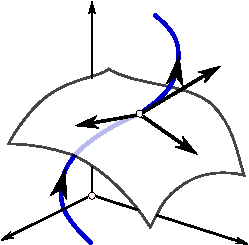
\includegraphics[width=\unitlength]{A28tangent3}}%
    \put(0.91612064,0.70682767){\color[rgb]{0,0,0}\makebox(0,0)[lb]{\smash{$\vel$}}}%
    \put(0.48698745,0.90266503){\color[rgb]{0,0,0}\makebox(0,0)[lb]{\smash{$\ssp(\zeit)$}}}%
    \put(0.2624318,0.5347756){\color[rgb]{0,0,0}\makebox(0,0)[lb]{\smash{$\groupTan_1$}}}%
    \put(0.80471037,0.38188675){\color[rgb]{0,0,0}\makebox(0,0)[lb]{\smash{$\groupTan_2$}}}%
    \put(0.538343,0.25344355){\color[rgb]{0,0,0}\makebox(0,0)[lb]{\smash{$\LieEl\ssp$}}}%
    \put(0.47864531,0.56060893){\color[rgb]{0,0,0}\makebox(0,0)[lb]{\smash{$\ssp$}}}%
  \end{picture}%
~~(b)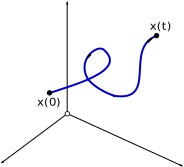
\includegraphics[width=0.20\textwidth]{A27traj}
\\
(c)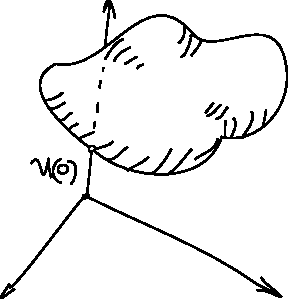
\includegraphics[width=0.20\textwidth]{A27gOrbit}
(d)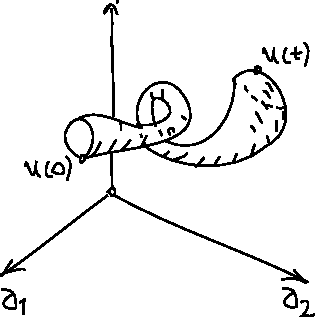
\includegraphics[width=0.20\textwidth]{A27wurst}
   \caption{\label{fig:A27wurst}
   (a)
In presence of $N$-continuous parameter symmetry, each \statesp\ point
$\ssp$ owns $(N\!+\!1)$ tangent vectors: one $\vel(\ssp)$ along the time
flow $\ssp(\zeit)$, and the $N$ group tangents  $\groupTan_1(\ssp), \,
\groupTan_2(\ssp) ,\,\cdots, \groupTan_N(\ssp)$ along infinitesimal
symmetry shifts, tangent to the group orbit $\LieEl\ssp$.
    (b)
Trajectory.
    (c)
Group orbit.
    (d)
Wurst.
}
\end{figure}
%%%%%%%%%%%%%%%%%%%%%%%%%%%%%%%%%%%%%%%%%%%%%%%%%%%%%%%%%%%%%%%%%%%%%

A flow $\map^t$ and the \statesp\ $\pS$ on which the flow acts comprise a
{dynamical system}. If a group $\Group$ of continuous transformations
acts on a continuous time flow, each \statesp\ point owns a set of
tangent vectors (\reffig{fig:A27wurst}\,(a)). Integrated globally, the
velocity vector $\vel(\ssp)$ traces out the {\em trajectory}
$\flow{\zeit}{\ssp}$ ( \reffig{fig:A27wurst}\,(b)). Applying the continuous
transformations traces out the {group orbit} (or, from now on, just
\emph{orbit})
\(
\pS_\ssp = \{\LieEl\,\ssp \mid \LieEl \in {\Group}\}
% \,,\qquad \pS_\ssp \subset \pS
\,
\) %ee{sspOrbit}
(\reffig{fig:A27wurst}\,(c)). Together they trace out a complicated smooth
manifold (hereafter affectionately referred to as the {\em wurst}, see
figures~\ref{fig:A27wurst}\,(d), \ref{fig:CLf01group}\,(b) and
\ref{fig:sliceimage}), that we shall teach you here how to slice.

A flow is said to have symmetry $\Group$ if the form of evolution
equations $\dot{\ssp} = \vel(\ssp)$ is left invariant,
\(
\vel(\ssp)=\LieEl^{-1} \, \vel(\LieEl \, \ssp)
% \,,\qquad \mbox{for all }
\,,
\) %ee{eq:FiniteRot}
by the set of transformations $\LieEl \in {\Group}$. Physicists love
symmetry, but Nature does not care: turbulence breaks all symmetries,
and while the flow equations may be invariant under $\Group$, their
solutions typically are not.

The key to chaotic dynamics is the notion of recurrence. To quantify how
close the state of the system now is to a previously visited state, we
need the notion of distance between two points in \statesp. The simplest
(but far from the only, or the most natural) is the Euclidean norm
\beq
  \Norm{\ssp-\ssp'}^2  = \braket{\ssp-\ssp'}{\ssp-\ssp'} =
\sum_j^d
(\ssp-\ssp')_j^2
\,.
\ee{innerproduct}
Given a notion of distance we can talk about 'neighborhood,' the open set of
nearby states. Our main task in what follows will be to make this precise,
by defining a chart over a neighborhood, and its borders.
Given distances and neighborhoods,
the next key notion is  \emph{measure}, or how likely a typical
trajectory is to visit a given neighborhood. After some observations of a
given turbulent flow, one can identify a set of representative
\emph{\template s}\rf{rowley_reconstruction_2000}, {points}
$\slicep{}^{(j)}$, $j=1,2,\cdots$ in the \statesp\ $\pS$, which are the
dynamically most important unstable {\recurrStr s} of the flow.
%    \DB{2012-04-12}{Neighborhoods not defined up to this point
%    in the text. Should they be? Predrag: done now.}

Our goals here are two-fold:
(i) In \refsect{s:cut} we review the method of \PoincSec s, with
    emphasis on aspects applicable to high-dimensional flows: construction of
    multiple local linear `charts' and determination of their borders and
(ii) in \refsect{s:slice} we show how the same set of tools applied to
    reduction of continuous symmetries enables us to commence a
    systematic charting of the long-time dynamics of high-dimensional
    flows with continuous symmetries (\refsect{s:chart}).

    \ifdraft\color{blue}
still to discuss:
\begin{itemize}

  % \item section {\PoincS} vs slice \pSRed

  \item strobing $\sim$ method of connections

  \item reduction vs projection
\end{itemize}
    \color{black}\fi

\PC{recheck PACS on the title page}
% history.tex
%
% Predrag created file              jul 3 2006
% $Author$ $Date$


\section{{\Rpo s} - a brief history}

The KS equation  \refeq{ks} is time translationally invariant,
and 
space translationally invariant
under the 1-$d$ Lie group of $O(2)$ rotations: if
$u(x,t)$ is a solution, then $u(x+d,t)$ is an equivalent
solution for any $-L/2 < d \leq L/2$.
As a result,
KS can have \rpo\ solutions with nonzero shift
\beq
u(x+d,\period{}) = u(x,0)
\,.
\ee{KSrpos}
where $\period{}$ is the period.
\ES{Is this obvious to everybody? I cannot really see why it is so.}


{\Rpo s} were introduced by Poincar\'e in his study of 
the 3-body problem\rf{ChencinerLink,rtb}.
% says Chenciner\rf{ChencinerLink}
Consider motion of a test particle of mass
$\mu \ll 1$ in the
restricted three-body problem,
under the
influence of the gravitational force of two heavy bodies with masses $1$ and
$\mu \ll 1$ fixed at $(-\mu,0)$ and $(1-\mu,0)$. \Reqva\ of this problem
are known as the Lagrange points. They are stationary in
the co-rotating frame, but
in the inertial frame they execute circular motions.
Similarly, in appropriate co-rotating frame
{\rpo s} are periodic orbits, 
but in the inertial frame their trajectories
are quasiperiodic. 
The \reqva\ and \rpo s 
respectively arise from
\eqva\ and periodic solutions of Hamiltonians reduced by symmetries.
They arise in dynamics of many physical systems
with continuous symmetries, such as motions of rigid bodies, gravitational
$N$-body problems, molecules and nonlinear waves.
A striking recent application of \rpo s has been the discovery
of ``choreographies" of $N$-body problems\rf{McC7,McC8,McC}.
%add \PC{some McCord references}

Lan has some \reqva\ (travelling waves) for KS in his
thesis\rf{Lan:Thesis}, %http://chaosbook.org/projects/theses.html
 and for complex LG in a paper on ``MAWs".
Viswanath\rf{ViswanathPC06} % arXiv.org/physics/0604062
found them in the plane Couette problem.

Here we determine 
several \eqva\ and many \rpo s for 
KS in a periodic cell of size $L=22$.


%\section{\KSe}
%\label{sec:KSe}

The \KS\ [henceforth KS] system was derived by
Kuramoto and Tsuzuki\rf{ku} as a phase equation for
reaction-diffusion systems described by Complex Ginzburg-Landau
equation and independently by Sivashinsky\rf{siv} to describe
instabilities in laminar flame fronts. It also appears
in a variety of contexts including thin falling
films and interfacial instabilities between
concurrent viscous fluids\rf{BenKS66,LinKS74}.
% For an instructive derivation from Complex Ginzburg-Landau
% equation \cf~\rf{}.
Our motivation for its study is that it is one of the simplest
nonlinear PDEs that exhibit features reminiscent of fluid
turbulence and thus it is a convenient system to test new ideas.

 In the formulation
adopted here, the time evolution of the `flame front velocity'
$u=u(x,t)$ %on a periodic domain $u(x,t) = u(x+L,t)$
is given by
\beq
  u_t = F(u) = -{\textstyle\frac{1}{2}}(u^2)_x-u_{xx}-u_{xxxx}
    \,,\qquad   x \in [-L/2,L/2]
    \,,
\ee{ks}
with appropriate boundary conditions, as discussed in \refsect{sec:KSbc}.
Here $t \geq 0$ is the time, and $x$ is the spatial coordinate.
The subscripts $x$ and $t$ denote partial derivatives with respect to
$x$ and $t$.

\subsection{Boundary conditions and system size}
\label{sec:KSbc}

Ideally we would like to work in a system of infinite spatial extend, \ie\ in the limit $L\rightarrow\infty$.
Although solutions of KS equations in this limit have appeared, \cf for example \refrefs{hooper_travelling_1988,feng_multiplicity_2004}\ES{More citations needed. Kevrekidis \etal\
mention criticism of periodic BC, but they give no reference.}, it is
more convenient, both computationally and theoretically, to work with periodic boundary conditions
\beq
  u(x,t) = u(x+L,t)\,,
 \label{eq:KSper}
\eeq
and this is the usual choice in the literature and the one followed in this thesis.
% The justification in terms of the physics
% of the problem is that we focus our attention to a small part of a larger system,
% far away from the boundaries. Further
Justification of this choice will be given
in \refsect{sec:KSeSymm}, in conjunction with the discussion of the symmetries of the system.

Another common choice of boundary conditions is
\beq
  u(0,t) = u(L,t)=0\,,
 \label{eq:KSodd}
\eeq
which restricts the system to the subspace of odd functions. This choice will also be discussed
in \refsect{sec:KSeSymm}.

In what follows
we shall state results of all calculations either in units of the system size $L$
or the `dimensionless system size' $\tildeL=L/2\pi$.
All numerical results presented in this thesis
are for $\tildeL=22/2\pi = 3.5014\ldots$, unless otherwise
noted. The system size leads to a system that is just ``turbulent'' enough
to have interesting dynamics, \cf \refsect{sec:L22}, while being still
rather tractable and can be used  as a test bed for
continuous symmetry reduction and a dynamical systems approach, see also \refsect{sec:ksSizeBC}.

\subsection{Symmetries of \KS\ system}
\label{sec:KSeSymm}

In an unbounded domain, $x\in(-\infty,\infty)$, KS equation is equivariant
under the action of the non-compact Euclidean group $\En{1}$:
If $u(x,t)$ is a solution, then
$\Shift({\shift})\, u(x,t) = u(x+\shift,t)$
is an equivalent solution for any shift
$\shift\in\Rls{}$, as is the reflection (`parity' or `inversion') $\Refl$ defined by
\beq
    \Refl \, u(x) = -u(-x)
\,.
\ee{KSparity}

Imposing periodic boundary conditions we restrict attention to the subspace
$[-L,L]$ in which only the compact subgroup \On{2} of \En{1} acts by:
\beq
	\Shift_{\shift/L}\, u(x,t) = u(x+\shift,t)\,,\qquad \shift\in\left[-L/2,L/2\right]	
	\label{KSshift}
\eeq
and reflections \refeq{KSparity}. Here we use subscript
notation for shifts to differentiate with the case of \En{1}.
Moreover, we only consider perturbations within this subspace,
\ie\ we do not consider subharmonic perturbations. The system
size $L$ affects the representation of \On{2}, \cf
\refsect{sec:fourKS}. \ES{This statement needs to be checked:
An important fact is that the isotropy subgroups of \En{1} (of
\En{n} in general) are all compact subgroups, if the action is
proper, see for example \refref{ChossLaut00}. Thus the
equivariant bifurcation structure as $L$ increases is not
affected, at least as long as we are not in the
spatio-temporally chaotic regime, when the spectrum of
stability eigenvalues becomes quasi-continuous.} Reflection
generates the dihedral subgroup $\Dn{1} = \{1, \Refl\}$ of
$\On{2}$. Boundary conditions \refeq{eq:KSodd} restrict the
system to \Fix{\Dn{1}} and thus in that case symmetry \Dn{1}
is impossed to all solutions. To avoid technical difficulties
associated with the action of \On{2} on an infinite dimensional
space we will discuss the isotropy subgroups of \On{2} in
\refsect{sec:ksIso}, after we truncate \refeq{expan} to finite
order.


The KS equation is also Galilean invariant: if $u(x,t)$ is a solution,
then $u(x -ct,t) -c $, with $c$ an arbitrary constant
speed, is also a solution. As one can verify by integrating \refeq{ks} with
respect to $x$ over the periodic domain $[-L/2,L/2]$ the quantity
 $\int_{-L/2}^{L/2} u\,dx$
is conserved and we can, without loss of generality, set it equal to zero. This corresponds
to the choice $c=0$, therefore eliminating Galilean invariance.


% $G$, the group of actions $ g \in G $ on a
% \statesp\ (reflections, translations, \etc) is a symmetry of the KS
% flow \refeq{ks} if $g\,u_t = F(g\,u)$.

% The KS equation is time translationally invariant, and space translationally invariant
% on a periodic domain under
% the 1-parameter group of
% $O(2): \{\Shift_{\shift/L},\Refl \}$.
% If $u(x,t)$ is a solution, then
% $\Shift_{\shift/L}\, u(x,t) = u(x+\shift,t)$
% is an equivalent solution for any shift
% $-L/2 < \shift \leq L/2$,
% as is the
% reflection (`parity' or `inversion')
% \beq
%     \Refl \, u(x) = -u(-x)
% \,.
% \ee{KSparity}

\subsection{Why $L=22$ on periodic domain?}
\label{sec:ksSizeBC}

For \KS\ system with periodic boundary conditions one expects to find
traveling wave (\reqv) and modulated amplitude traveling wave
(\rpo) solutions, exactly the kind of
solutions that we set out to understand and organize. Indeed,
a very detailed bifurcation study of such solutions for \KSe\
has been carried out by Brown and Kevrekidis\rf{BrKevr96},
see discussion in \refsect{sec:KSePO}. In our work the emphasis is
on working with a specific system size, with specific boundary
conditions, and determining and labeling all unstable periodic
and relative periodic solutions (up to a given topological
length). A bifurcation analysis is not practical for
such a task as global bifurcations that lead to creation and
disappearance of (relative) \po s are hard to track.
Therefore one needs to understand the geometry of phase space
in order to detect and organize the compact solutions
systematically.

The \KS\ system of size $L=22$ appears amenable to such a
geometric study, yet it provides new challenges. As we will
see in \refchap{chap:kseStSp}, many of the invariant objects
(\eqva, \reqva, {\po s}, {\rpo s}) have more than one
unstable eigendirections, a situation that has not been dealt
with in previous \KSe\ studies in terms of periodic
orbits\rf{Christiansen97,LanThesis,lanCvit07}, and which very
often occurs in the studies of \pCf\
\rf{GHCW07,HGC08,GHCV08,HalcrowThesis}. Nevertheless, the
system is not large enough to exhibit many unstable,
essentially non-separated (quasi-continuous) eigenvalues.
Systems with quasi-continuous spectra are known as
\emph{spatio-temporally chaotic} in the sense that they are
disordered both in space and in
time\rf{manneville_instabilities_2004} and a dynamical
description of such systems presents many more challenges
than we would like to be faced with while we try for the
first time to understand the organization of a flow in terms
of (modulated) traveling wave solutions.  The $L=22$ system
remains within reach of a dynamical description, see
\refchaps{chap:kseStSp}{chap:kseRedStSp}, while offering
valuable insight on how to deal with other, larger, more
turbulent or realistic systems.




\subsection{Fourier space}
\label{sec:fourKS}

\On{2} equivariance makes it convenient to work in Fourier space,
\beq
  u(x,t)=\sum_{k=-\infty}^{+\infty} a_k (t) e^{ i k x /\tildeL }
\,,
\ee{eq:ksexp}
with the $1$-dimensional PDE \refeq{ks}
replaced by an infinite set of
ODEs for the complex Fourier coefficients $a_k(t)$:
\beq
\dot{a}_k= \pVeloc_k(a)
     = ( q_k^2 - q_k^4 )\, a_k
    - i \frac{q_k}{2} \sum_{m=-\infty}^{+\infty} a_m a_{k-m}
\,,
\ee{expan}
where $q_k = k/\tildeL$.
Since $u(x,t)$ is real,
 \beq
  a_{k}=a^\ast_{-k} \,,
  \label{eq:astar}
 \eeq
and we can replace the
sum by a $k > 0$ sum. Note that $\dot{a}_0=0$ in
 \refeq{expan} as a result of Galilean invariance and $a_0$ is a conserved quantity
 fixed to $a_0=0$ by the condition $\int_{-L/2}^{L/2} u\,dx$=0.
In the Fourier basis \On{2} acts absolutely irreducibly on each complex plane
$\left(\Re(a_k),\Im(a_k)\right)$ and the linear part of \refeq{expan} is conveniently
diagonalized. Indeed, the translation operator action on the Fourier coefficients \refeq{eq:ksexp},
represented here by a complex valued vector
$a = \{a_k\in\mathbb{C}\,|\,k = 1, 2, \ldots\}$, is given by
\beq
  \Shift_{\shift/L}\, a = \mathbf{g}(\shift) \, a \,,
  \label{eq:shiftF}
\eeq
where $\mathbf{g}(\shift) = \mathrm{diag}( e^{i q_k\, \shift} )$ is a complex
valued diagonal matrix, which amounts to the $k$-th mode complex plane
rotation by an angle $k\, \shift /\tildeL$. The reflection acts on
the Fourier coefficients by complex conjugation and a change of sign,
\beq
  \Refl \, a = -a^\ast
\,.
\label{eq:FModInvSymm}
\eeq

\ES{This is from my first year KS special problem, perhaps some parts are usable:
Some qualitative comments about the KS equation can now be easily
given in view of \refeq{expan}. The linear behavior of the system
depends on the sign of the quantity $k^2- \left(2\pi/L\right)  k^4$.
For a sufficiently large system, the first few values of $k$ yield $k^2- \left(2\pi/L\right)
k^4>0$ or $k<\sqrt{L/2\pi}$ and the corresponding Fourier components grow exponentially
with time (unstable components). In other words the anti-diffusion
term in \refeq{eq:KS} (resulting in the term $\sim k^2$ in
\refeq{eq:Fcoef}) dominates over the dissipation term (resulting in
$\sim k^4$ in \refeq{eq:Fcoef}).  On the other hand there are infinitely many larger
wavenumber components with $k>\sqrt{L/2\pi}$ for which the solutions
are bounded (stable components). The role of the bilinear term in
\refeq{eq:Fcoef} is then to excite the larger wavenumber components
while dissipating the smaller wavenumber ones. The result of this
competition is that the asymptotic dynamics of the system are
confined on a low dimensional attractor.}


\subsection{Truncation}

Dynamical \statesp\ representation of a PDE is $\infty$-dimensional,
but the KS flow is strongly contracting and its non-wondering set,
and, within it, the set of invariant solutions investigated here, is
embedded into a finite-dimensional inertial manifold\rf{FNSTks85} in
a non-trivial, nonlinear way. The existence of an inertial manifold for
\KSe with both odd and periodic boundary conditions has been proved and
several bounds for its dimension have been found, \cf\ \refref{jolly_evaluating_2000} and references
therein. The best current bound in dimension of inertial manifold for KS
equation with periodic boundary condition is, to the author's knowledge,
given in \refrefs{Robinson_inertial_1994,jolly_evaluating_2000}: $O(L^{2.46})$ for $L\in[2\pi,6\pi]$.

The fact that the asymptotic dynamics lies on a finite
dimensional manifold justifies truncation of the infinite tower
of equations \refeq{expan} to finite order $N$. According to
the bound $O(L^{2.46})\simeq2000$ for $L=22$\ES{$L=22>6\pi$, so
it looks like their proof does not apply to our system if one
wants to be rigorous.} and we would expect to need even more
Fourier modes, since the Fourier basis is not directly
connected to coordinates on the inertial manifold of KSe and
would therefore be less optimal than an approach that
approximates such coordinates, for
example\rf{Jolly_approximate_1990,JRT01}.
Nevertheless such a bound seems rather inflated compared to
numerical simulations of the asymptotic dynamics that typically
require $O(10)-O(100)$ Fourier modes. In practice we keep
$16\leq N \leq 128$ Fourier modes in numerical simulations and
check the robustness of the results against increase of $N$.

\subsection{Isotropy lattice and invariant subspaces}
\label{sec:ksIso}

Let $N$ be the number of Fourier modes retained in \refeq{expan}
and observe that the action of $O(2)$
on \Rls{N} by \refeq{eq:shiftF} and \refeq{eq:FModInvSymm} is,
up to the minus sign in \refeq{eq:FModInvSymm}, identical
to the action \refeq{eq:O2stndrd} of \On{2} on \Clx{N} studied
in \refsect{sec:strata}.
The isotropy lattice remains unchanged but \fixedsp s of the dihedral subgroups are affected.
\Fixedsp s of \Cn{q}, given by the condition
\beq
	a_k=0\ \mathrm{unless}\ k = q j\,,\ j=1,\ldots\lfloor n/q \rfloor\,,
	\label{eq:O2ksCqFix}
\eeq
remain unchanged but the \fixedsp s of the dihedral subgroups \Fix{\Dn{m}} are now given by the conditions
\bea
	a_k=0\ \mathrm{unless}\ k = m j\,,\ j=1,\ldots\lfloor n/m \rfloor\,, \\
	\Re(a_k)=0\ \mathrm{for}\ k=1,\ldots,n\,.
	\label{eq:O2ksDqFix}
\eea
In relation to physical space we observe that \Fix{\Dn{1}} is the subspace of antisymmetric functions $Re(z_k)=0,\, \forall k$ or $u(-x)=-u(x)$ while for the action \refeq{eq:O2stndrd} the corresponding
subspace would be that of symmetric functions.

\subsection{\Eqva\ and their bifurcations}
\label{sec:ksBif}

%%%%%%%%%%%%%%%%%%%%%%%%%%%%%%%%%%%%%%%%%%%%%%%%%%%%%%%%%%%%%%%%%%
\begin{figure}[ht]
\begin{center}
  (\textit{a})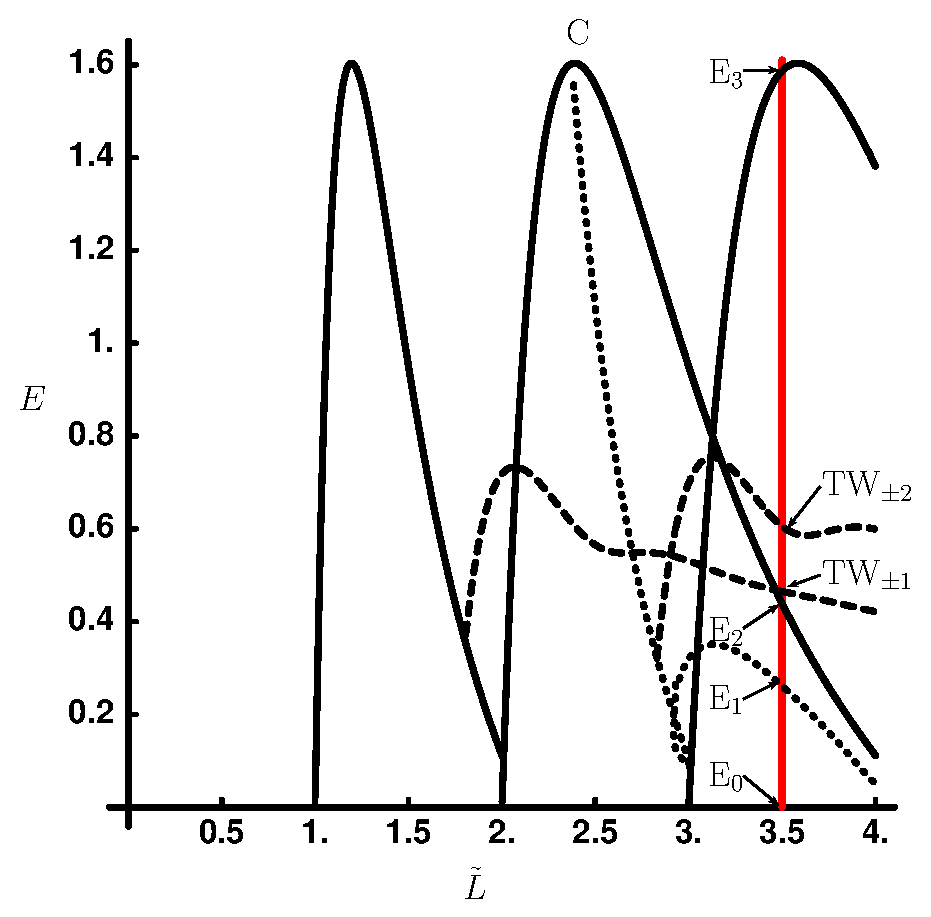
\includegraphics[width=0.5\textwidth]{../figs/ksBifDiag}
\end{center}
\caption[KS steady state bifurcations]{
The energy \refeq{ksEnergy} of the \eqva\ and \reqva\ that
exist up to $L=22$, $\tildeL = 3.5014\ldots$, plotted as a function
of the system size $\tildeL = L/2\pi$ (additional \eqva, not present
at $L = 22$ are given in \refref{ksgreene88}). Solid curves denote
$n$-cell solutions \EQV{2} and \EQV{3}, dotted curves the GLMRT
\eqv\ \EQV{1},
and dashed curves the \reqva\ \REQV{\pm}{1} and \REQV{\pm}{2}.
The parameter $\alpha$ of \refrefs{KNSks90,ksgreene88} is
related to the system size by $\tildeL=\sqrt{\alpha/4}$.    }
\label{fig:ksBifDiag}
\end{figure}
%%%%%%%%%%%%%%%%%%%%%%%%%%%%%%%%%%%%%%%%%%%%%%%%%%%%%%%%%%%%%%%%

\Eqva\  (or the steady solutions)
are the fixed profile time-invariant solutions,
\beq
 u(x,t) = u_\stagn(x)
\,.
\ee{eqva}
Due to the translational symmetry,
the KS system also allows for
\reqva\ (traveling waves, rotating waves),
characterized by a fixed profile $u_\stagn(x)$
moving with constant speed $c$, {\ie}
\beq
 u(x,t) =  u_\stagn(x-ct)
\,.
\ee{reqva}
Here suffix ${}_\stagn$ labels a particular invariant solution.
Because of the reflection symmetry \refeq{KSparity},
the \reqva\ come in counter-traveling pairs
$u_\stagn(x-ct)$, $-u_\stagn(-x+ct)$.

The \reqv\ condition for the {\KS} PDE \refeq{ks}
is the ODE
\beq
{\textstyle\frac{1}{2}}(u^2)_x+u_{xx}+ u_{xxxx}=c \, u_x
\ee{KSeqvCond}
which can be analyzed as a dynamical system in its own right.
Integrating once we get
\beq
{\textstyle\frac{1}{2}}u^2 - c u + u_x + u_{xxx}=\expctE
\,.
\label{eq:stdks}
\eeq
This equation can be interpreted as a 3-dimen\-si\-on\-al dynamical system
with spatial coordinate $x$ playing the role of `time,'
and the integration constant \expctE\ can be interpreted as `energy,'
see \refsect{sec:energy} and \reffig{fig:ksBifDiag}.

In the Fourier representation the \reqva\ time dependence is
\beq
 a_k(t) e^{-itc q_k} = a_k(0)
\,.
\ee{reqvaF}
Differentiating with respect to time, we obtain
the Fourier space version of the \reqv\ condition
\refeq{KSeqvCond},
\beq
 \pVeloc_k(a) - i q_k c a_k = 0
\,,
\ee{reqvCondF}
which we solve for (time independent) $a_k$ and $c$, see \refchap{chap:kseStSp}.

In a periodic box of size $L$
both \eqva\ and \reqva\ are  periodic solutions
embedded in 3-$d$ space, conveniently represented as loops in
$(u,u_x,u_{xx})$ space, see \reffig{f:KS22Equil}\,(\textit{d}).
In this representation the continuous translation symmetry
is automatic -- a rotation in the $[0,L]$ periodic domain only
moves the points along the loop. For an \eqv\ the points
are stationary in time; for \reqv\ they move in time, but in
either case, the loop remains invariant.
% So we do not have the problem that we encounter in the Fourier
% representation, where seen from the frame of one of the \eqva\
% the rest trace out circles under the action of continuous symmetry
% translations.
Unfortunately this visualization has not helped
our understanding of \KSe\ state space.

The  \eqva\ and \reqva\ of KS equation and their bifurcations have been
the object of extensive study and a literature survey
cannot be exhaustive. The results of relevance for this thesis can be
found in \refrefs{Mks86,laquey74,ksgreene88,KNSks90,AGHks89}.
Although these results were obtained by direct bifurcation
analysis rather than with methods of equivariant
bifurcation theory, the relation of bifurcations to \On{2}
symmetry has been recognized in the literature particularly in
\refrefs{KNSks90,AGHks89}. The relation of the bifurcations
found numerically (and in some cases analytically) in
\refref{KNSks90} to the predictions of equivariant bifurcation
theory is discussed in Krupa\rf{Krupa90} but
without explicit calculations. In this section we describe some
of the elementary and well known bifurcations in KS equation
from the point of view of equivariant bifurcation theory.

 Since the origin (u(x,t)=0 in physical space) is the \fixedsp\ of \On{2} it is,
by \refPro{pro:gfInv}, flow invariant and thus
an \eqv. From commutation relation \refeq{eq:LrzCommut} we conclude that the
linear stability matrix (see \refsect{sec:ksReal}) $A(0)$
and the representation of the symmetry group \On{2} share a complete
set of eigenvectors, the Fourier modes.
% From relation \refeq{eq:LrzCommut} $A(0)$ has to commute
% with the generator of rotations, which in real Fourier basis becomes
% \beq
% \begin{array}{lll}
%  & × & × \\
% × & × & × \\
% × & × & ×
% 	  \end{array}
% \)
% \eeq
Moreover, since \On{2} acts absolutely irreducibly
on each Fourier plane $A(0)$ is diagonal (in real Fourier basis)
with eigenvalues $\lambda_0^{(k)}=( q_k^2 - q_k^4 )$, from \refeq{expan}.
For $L<2\pi$
the origin is linearly stable and due to the hyperviscous damping $u_{xxxx}$ it is the global
attractor\rf{KNSks90}. At $L=2\pi$ the origin loses stability and due
to the diagonal form of $A(0)$ the kernel of the linearization is immediately seen to be the
$k=1$ irreducible subspace. Taking into account the orthogonality of the Fourier basis, the Lyapunov-Schmidt reduction \cite{golubitsky2002sp} is automatic and we can work in the $k=1$ subspace (\cf ``Restriction Lemma'' in \refref{KNSks90}
for technical details). In this subspace all requirements
of Equivariant Branching Lemma \cite{golubitsky2002sp}\ES{write, add refThe.} are satisfied: $\On{2}$ acts
absolutely irreducibly, $v_1(a)$ is equivariant (Lyapunov-Schmidt reduction respects symmetry),
the eigenvalue crossing condition holds $\frac{d}{d L}\lambda_0^{(1)}(2\pi)\neq 0$, and
finally $\Dn{1}$ is an axial subgroup since \Fix{\Dn{1}} is the imaginary axis in the complex $a_1$ plane.
Therefore there is a unique solution branch of \eqva\ in \Fix{\Dn{1}}, \ie\ with symmetry $\Dn{1}$.
% \ES{After secondary bifurcations it appears that the branch does not remain in \Dn{1}, check.}
This is known as the unimodal branch in the literature. The stability of the bifurcating \eqv\
can not be determined from symmetry arguments and one has to take into account the evolution equations
\refeq{expan}. The unimodal \eqv\ is stable at bifurcation\rf{KNSks90}. Under the action of $\Shift$ we
get a continuous family of \eqva\ for any \eqv\ in $D_1$.

The bifurcation scenario repeats itself each time $L=2\pi k$: The $k$'th mode eigenvector of
the origin looses stability and an \eqv\ with symmetry $D_k$ is born, giving rise to
the $k$-modal branch. The Lyapunov-Schmidt reduction and application of Equivariant branching lemma
carries through in exactly the same way. In \refref{KNSks90} the observation is made that one
can get the k-modal branch from the unimodal through the substitution $u(x)\mapsto u(kx)$
and therefore the $k$-modal branches are called k-fold replications
of the unimodal branch, \cf\ also \refref{Krupa90}. Note that the k-modal branch
with $k>1$ ``inherits'' the unstable directions of the origin and thus are born unstable at the
bifurcation. In \refref{ksgreene88} states in the $k$-modal branch are called $k$-cell states.
Condition \refneq{eq:O2ksDqFix} implies that in these states only the Fourier modes $a_j$ where $j$
is a multiple of $k$ are non zero. Each $k$-modal branch merges with the $2k$-modal branch, see \reffig{fig:ksBifDiag}
and \refrefs{KNSks90,ksgreene88}. Note that, according to \refexam{O2iso}, $\Fix{\Dn{1}}\supset\Fix{\Dn{k}}$
for all $k$, so all unimodal \eqva\ are antisymmetric.

The replication observed in primary bifurcations is not carried to the secondary bifurcations that are
much richer. From here on we only consider bifurcations that play a role in the dynamics for our system size, $L=22$, see \reffig{fig:ksBifDiag}. The $\EQV{2}$ and $\EQV{3}$ indicated in that diagram belong
in the bimodal and trimodal branches, respectively.

The $1$-cell state loses stability and bifurcates to a branch of stable
\reqva, which later on becomes unstable through a Hopf bifurcation\rf{KNSks90,ksgreene88}.
This is the branch indicated as $\REQV{\pm}{1}$ in \reffig{fig:ksBifDiag}. Since \reqva\ are not in \Fix{\Dn{1}}
and they are invariant, as a set, under translations \refneq{eq:shiftF}, they have to come in copies
under the action of \Dn{1}. The sign in $\REQV{\pm}{1}$ indicates direction of rotation, see \refeq{reqva}.
\PublicPrivate{}{For a discussion of relation of this bifurcation to Krupa's theorem, see \refref{Krupa90}.}%end \PublicPrivate

At point $C$ in \reffig{fig:ksBifDiag} the $2$-cell state
bifurcates to a type of \eqv\ solution found by La Quey,
Mahajan, Rutherford and Tang\rf{laquey74} and generalized by
Greene and Kim who refer to them as GLMRT \eqva. In
\refref{KNSks90} this branch of solutions is refered to as
bi-tri branch as it is later on terminated at the trimodal
branch. Bi-tri \eqva\ live in \Fix{\Dn{1}} and have components
in all Fourier modes\ES{Is this symmetry increasing
bifurcation?}. At the point where the bi-tri branch meets the
trimodal branch a new branch is born that is still in
\Fix{\Dn{1}}. This is seen as a continuation of the bi-tri
branch in \refref{KNSks90}. The \eqv\ labeled \EQV{1} in
\reffig{fig:ksBifDiag} is in this branch.

Finally the \reqv\ that is labeled \REQV{\pm}{2} belongs to a branch bifurcating from the bi-tri branch in
a Hopf bifurcation. Once again the \reqva\ come in \Dn{1} related, counter-traveling pairs.


% \ES{I think there is a symmetry we have missed. It looks like the unstable eigenvectors of
% \EQB{3} are in \Cn{3} on which rotations act and therefore after reduction we get one unstable
% eigendirection. This explains the multiplicity of the eigenvalue and maybe the shape of its
% unstable manifold.}


\PublicPrivate{}{

For $\expctE>0$ there is rich
$\expctE$-dependent dynamics, with
fractal sets of bounded solutions investigated in
depth by Michelson\rf{Mks86}.
For $\tildeL<1$ the only \eqv\ of the system is the
globally attracting constant
solution $u(x,t)=0$, denoted $\EQV{0}$ from now on. With increasing system size $L$ the system
undergoes a series of bifurcations.
The resulting \eqva\ and
\reqva\ (but not \po s and \rpo s)
are described in the classical papers of
Kevrekidis, Nicolaenko and Scovel\rf{KNSks90},
and Greene and Kim\rf{ksgreene88}.
The relevant bifurcations
up to the system size
investigated here are summarized
in \reffig{fig:ksBifDiag}:
at $\tildeL=22/2\pi =
3.5014\cdots$, the {\eqva} are the constant solution
\EQV{0}, the GLMRT\rf{laquey74,ksgreene88} \eqv\ \EQV{1}, the $2$-
and $3$-cell states \EQV{2} and \EQV{3},
and the pairs of \reqva\ \REQV{\pm}{1}, \REQV{\pm}{2}.

Periods of spatially periodic {\eqva} are multiples of $L$.
Every time the system size crosses  $\tildeL=n$,
$n$-cell states
are generated through pitchfork bifurcations off $u =0$
\eqv.
Due to the translational invariance of {\KSe},
they form invariant circles
in the full \statesp.
In the $\bbUplus$ subspace considered here,
they correspond to $2n$ points, each shifted by $L/2n$.
For a sufficiently small $L$
the number of {\eqva} is small and
concentrated on the low wave-number end of the Fourier spectrum.

From \refeq{expan} we see that the origin $u(x,t) = 0$
has Fourier modes as the linear stability eigenvectors
(see Appendix~\ref{sec:stability}).  The $|k|<\tildeL$
long wavelength perturbations of the flat-front {\eqv}
are linearly unstable, while all
$|k|> \tildeL$ short wavelength perturbations are strongly contractive.
The high $k$ eigenvalues, corresponding to rapid variations of
the flame front, decay so fast that the corresponding eigendirections
are physically irrelevant.
The most unstable mode, nearest to $|k|=\tildeL/\sqrt{2}$,
sets the scale of the mean wavelength $\sqrt{2}$
of the KS `turbulent' dynamics,
see \reffig{f:ks_largeL}.
}%end \PublicPrivate



\subsection{\Rpo s and \po s} \label{sec:KSePO}

% The KS equation \refeq{ks} is time translationally invariant, and
% space translationally invariant under the 1-$d$ Lie group of $O(2)$
% rotations: if $u(x,t)$ is a solution, then $u(x+\shift,t)$ and
% $-u(-x,t)$ are equivalent solutions for any $-L/2 < \shift \leq
% L/2$.
As a result of invariance under $\Shift_{\shift/L}$,
KS equation can have \rpo\ solutions
with a profile $u_p(x)$, period $\period{p}$, and a
nonzero shift $\shift_p$
\beq
  \Shift_{\shift_p/L}u(x,\period{p}) =
  u(x+\shift_p,\period{p}) = u(x,0) = u_p(x)\,.
\label{KSrpos}
\eeq
{\Rpo s} \refeq{KSrpos} are periodic in
$v_p=\shift_p/\period{p}$ co-rotating frame (see
\reffig{f:MeanVelocityFrame}), but in the stationary frame their
trajectories are quasiperiodic.  Due to the reflection symmetry
\refeq{KSparity} of KS equation, every {\rpo} $u_p(x)$ with shift
$\shift_p$ has a symmetric partner $-u_p(-x)$ with shift $-\shift_p$.
In Fourier space we have:
\beq
  {\bf g}(\shift_p)f^\period{p}(a_p) - a_p = 0\,,
\ee{eq:system}
with ${\bf g}$ as in \refeq{eq:shiftF}.

\PublicPrivate{}{
As $\shift$ is continuous in the interval $[-L/2, L/2]$,
the likelihood of a \rpo\ with $\shift_p = 0$ shift is zero,
unless an exact periodicity is enforced by a discrete symmetry,
such as the dihedral symmetries discussed above.
If the shift $\shift_p$ of a \rpo\ with period $\period{p}$ is such
that $\shift_p /L$ is a rational number, then the orbit is
periodic with period $n\period{p}$.  The likelihood to find such \po s is
also zero.
}

KS equation can also have periodic solutions
characterized by a profile $u_p(x)$,
and period $\period{p}$. In terms of symmetry it is easier to think of them
in (truncated) Fourier space. For any discrete\footnote{Recall from \refExa{O2iso} that \On{2} fixes the origin, so
we cannot have periodic orbits with spatial symmetry \On{2}.} subgroup in the isotropy lattice
we can have periodic solutions with spatial symmetry \Dn{k} or \Cn{k}. For all $\gamma$ in \Dn{k} or \Cn{k}.
\beq
  \gamma a_p(t) = a_p(t)\,, \qquad  \forall t\in[0,\period{p}]\,.
\eeq
Such a solution lives in \Fix{\Dn{k}} of \Fix{\Cn{k}}.
% or in the terminology of Golubitsky and Stewart\rf{golubitsky2002sp},
% it has spatial symmetry \Dn{k}.
The periodic orbits found in \refrefs{Christiansen97,lanCvit07}, for example,
are all in \Fix{\Dn{1}}, as a result of restricting the dynamics to that subspace by the choice of antisymmetric
boundary conditions. In our case, for $L=22$, the dynamics in \Fix{\Dn{1}} are dominated by attracting (within
the subspace) heteroclinic connections and thus we have no periodic orbits of this type, or in
any other of the \Fix{\Dn{k}} subspaces, see \refchap{chap:kseStSp}. Moreover spatial symmetries have to
be in the isotropy lattice, see Chapter~3 of \refref{golubitsky2002sp} so there are no more possibilities
for orbits with just spatial symmetry.

The second type of periodic orbits would have spatio-temporal symmetry
with spatial part a discrete subgroup in the isotropy lattice
$\stab{a_p(t)}=\Dn{k}$ or \Cn{k} and trivial spatial symmetry.
% In the terminology of Chapter~3 of \refref{golubitsky2002sp} we would
% say that the spatial part of the spatio-temporal symmetry is
% \Dn{k} or \Cn{k} and there are no spatial symmetries.
Yet, due
to algebraic restrictions on possible spatio-temporal
symmetries, see Chapter~3 of \refref{golubitsky2002sp}, the
spatial part has to be cyclic and thus we are left with
$\Dn{1}$ and $\Cn{k}$ as our possibilities. For our system
size, $L=22$, we have found no periodic orbits with isotropy
subgroup $\Cn{k}$, see \refchap{chap:kseStSp}. We have found
periodic orbits with isotropy subgroup $\Dn{1}$, period
$\doubleperiod{p}$, which satisfy
\beq
	\Refl a(t+\period{p})=a(t)\,,
	\label{eq:ppo}
\eeq
where $\period{p}=\doubleperiod{p}/2$ by the relation $\kappa^2=e$. We choose to label those
periodic orbits with the half-period $\period{p}$ because this will be the period in the $O(2)$-reduced space,
where the segment of the orbit for time $[\period{p},\doubleperiod{p}]$ is a repeat of the \emph{prime} segment
for $[0,\period{p}]$. Thus we will refer to those orbits as pre-periodic of period $\period{p}$.
Periodic orbits \refeq{eq:ppo} live in the principal stratum and thus their group orbit under translations \refeq{eq:shiftF} is a manifold of equivalent solutions. Returning to physical space we have
\beq
  \Refl u(x+\shift,\period{p}) =
  -u(-x-\shift,\period{p}) = u(x+\shift,0) = u_p(x)
  \,,
\label{KSpos}
\eeq
the family of equivalent solutions
parameterized by $\shift$
(as the choice of the reflection point is arbitrary,
the shift can take any value in $-L/2 < \shift \leq L/2$).
\PublicPrivate{}{
However, due to the KS equation invariance under reflection \refeq{KSparity},
two types of \po s are possible:

{\bf (a)} The \po\ lies within the  $\bbUplus$ antisymmetric subspace,
$-u_p(-x) = u_p(x)$, and $u(x,\period{p}) = u(x,0) = u_p(x)$.

{\bf (b)} If an
orbit is of reflection type \refeq{KSpos},
$\Refl\Shift_{\shift/L} u(x,\period{p}) =
-u(-x-\shift,\period{p}) = u(x,0)$, then it is
pre-periodic to a \po\ with period
$2\period{p}$.
Indeed, since $(\Refl\Shift_{\shift/L})^2 = \Refl^2 = 1$,
 and the KS solutions
are time translation invariant, it follows
from \refeq{KSpos} that
\[
  u(x,2\period{p}) = \Refl\Shift_{\shift/L} u(x,\period{p}) =
  (\Refl\Shift_{\shift/L})^2 u(x,0) = u(x,0)\;.
\]
Thus any shift acquired during time $0$ to
$\period{p}$ is compensated by the opposite shift during
evolution from $\period{p}$ to $2 \period{p}$.
}% end PublicPrivate
Such pre-periodic orbits
are a hallmark of any dynamical system with a discrete
symmetry, where they have a natural
interpretation as \po s in the
fundamental domain\rf{CvitaEckardt,DasBuch}.

Brown and Kevrekidis\rf{BrKevr96} study bifurcations branches
of \rpo s for a wide range of system sizes $L$ for \KSe. For
our system size they identify two \rpo\ branches.
They are
created when either a heteroclinic cycle (see \refchap{chap:kseStSp})
or \reqv\ becomes unstable, see also \refrefs{Krupa90,AGHO288,AGHks89}.
In \refref{BrKevr96} partially hyperbolic invariant tori are also found
for larger systems, see \refchap{chap:tobedone}.

\section{Energy transfer rates}
\label{sec:energy}

In physical settings where the observation times are much longer than
the dynamical `turnover' and Lyapunov times (statistical mechanics,
quantum physics, turbulence) periodic orbit theory\rf{DasBuch} provides
highly accurate predictions of measurable long-time averages such as
the dissipation and the turbulent drag\rf{GHCW07}. Physical predictions have to be
independent of a particular choice of ODE representation of the PDE
under consideration and, most importantly, invariant under all
symmetries of the dynamics. In this section we discuss a set of such
physical observables for the  1-$d$ KS invariant under reflections and
translations. They offer a representation of dynamics in which the
symmetries are explicitly quotiented out. We shall use these observable in
\refsect{sec:energyL22} in order to visualize a set of solutions on
these coordinates. They implement
symmetry reduction, but their utility, as we will see in \refsect{sec:energyL22},
has been limited.

The {space average} of a function $\obser = \obser(\pSpace,t) = \obser(u(x,t))$  on
the interval $L$,
\beq
    \expct{\obser} = \Lint{\pSpace}\, \obser(\pSpace,t)
    \,,
    \label{rpo:spac_ave}
\eeq
is in general time dependent.
Its mean value is given by the {time average}
\beq
\timeAver{\obser}
    =
\lim_{t\rightarrow \infty} \frac{1}{t} \int_0^t \! d\tau \, \expct{\obser}
    =
\lim_{t\rightarrow \infty} \frac{1}{t} \int_0^t \!
    \Lint{\tau}  d\pSpace\, \obser(\pSpace,\tau)
    \,.
\label{rpo:tim_ave}
\eeq
The mean value of $\obser = \obser(u_\stagn) \equiv \obser_\stagn$ evaluated on $q$
\eqv\ or {\reqv} $u(\pSpace,t) = u_\stagn(\pSpace-ct)$ is
\beq
\timeAver{\obser}_\stagn = \expct{\obser}_\stagn = \obser_\stagn\,.
\label{rpo:u-eqv} \eeq Evaluation of the infinite time average
\refeq{rpo:tim_ave} on a function of a \po\ or \rpo\
$u_p(\pSpace,t)=u_p(\pSpace,t+\period{p})$ requires only a single
$\period{p}$ traversal,
\beq
  \timeAver{\obser}_p = \frac{1}{\period{p}}
    \int_0^{\period{p}} \! d\tau \, \expct{\obser}
\,.
\label{rpo:u-cyc}
\eeq

Equation \refeq{ks} can be written as
\beq
    u_t=- V_x
        \,,\qquad
    V(x,t)={\textstyle\frac{1}{2}}u^2+u_{x} + u_{xxx}
    \,.
\ee{ksPotent} If $u$ is `flame-front velocity' then \expctE, defined in
\refeq{eq:stdks}, can be interpreted as the mean energy density.
So, even though KS is a phenomenological
small-amplitude equation, the time-dependent quantity
\beq
    \expctE=
  \Lint{\pSpace}
  V(x,t)=
  \Lint{\pSpace} \frac{u^2}{2}
  \label{ksEnergy} \eeq
has a physical interpretation\rf{ksgreene88} as the average `energy'
density of the flame front. This analogy to the mean kinetic energy
density for the Navier-Stokes motivates what follows.

The energy \refeq{ksEnergy} is intrinsic to
the flow, independent of the particular ODE basis set
chosen to represent the PDE. However, as the Fourier
amplitudes are eigenvectors of the translation operator,
in the Fourier space the energy is a diagonalized
quadratic norm,
\beq
\expctE
          =  \sum_{k=-\infty}^{\infty} E_k
\,,\qquad
E_k =
    {\textstyle\frac{1}{2}}|a_k|^2
\,,
\ee{EFourier}
and explicitly invariant term by term
under translations
\refeq{eq:shiftF}
and reflections \refeq{KSparity}.

Take time derivative of the energy density \refeq{ksEnergy},
substitute \refeq{ks} and integrate by parts. Total derivatives vanish
by the spatial periodicity on the $L$ domain:
\bea
   \dot{\expctE} &=&
     \expct{u_t \, u}
         = - \expct{\left({u^2}/{2} + u \, u_{x} + u \, u_{xxx}\right)_x u }
    \continue
    &=&
\expct{ u_x \, {u^2}/{2} + u_{x}{}^2 + u_x \, u_{xxx}}
    \,.
\label{rpo:ksErate}
\eea
The first term in \refeq{rpo:ksErate} vanishes by
integration by parts,
\(
3 \expct{ u_x \, u^2}= \expct{(u^3)_x} = 0
\,,
\)
and integrating the third term by parts yet again
one gets\rf{ksgreene88} that the energy variation is
\beq
   \dot{\expctE} = P - D
                \,,\qquad
      P =  \expct{u_{x}{}^2}
                \,,\quad
      D =  \expct{u_{xx}{}^2}\,.
\ee{EnRate}
The power $P$ pumped in by anti-diffusion $u_{xx}$ is
balanced by the energy dissipation rate $D$ due
hyper-viscosity $u_{xxxx}$ in the KS equation \refeq{ks}.

The time averaged energy density  $\timeAver{E}$
computed on a typical orbit goes to a constant, so
the expectation values \refeq{rpo:EtimAve} of drive and dissipation
exactly balance each out:
\beq
    \timeAver{\dot{E}}  =
    \lim_{t\rightarrow \infty}
        \frac{1}{t} \int_0^t d\tau \, \dot{\expctE}
=
      \timeAver{P} - \timeAver{D}
= 0
    \,.
\ee{rpo:EtimAve}
In particular, the \eqva\
and \reqva\ fall onto the diagonal in \reffig{f:drivedrag},
and so do time averages computed on \po s and \rpo s:
\beq
\timeAver{E}_p =
\frac{1}{\period{p}} \int_0^\period{p}d\tau \, E(\tau)
    \,,\qquad
\timeAver{P}_p =
\frac{1}{\period{p}} \int_0^\period{p} d\tau \, P(\tau)
    =
      \timeAver{D}_p
    \,.
\label{poE}
\eeq
In the Fourier basis \refeq{EFourier} the conservation of energy on average
takes form
\beq
0 = \sum_{k=-\infty}^{\infty} ( q_k^2 - q_k^4 )\,
    \timeAver{E}_k
\,,\qquad
E_k(t) =  {\textstyle\frac{1}{2}} |a_k(t)|^2
\,.
\ee{EFourier1}
The large $k$ convergence of this series is insensitive to the
system size $L$; $\timeAver{E_k}$ have to decrease much faster than
$q_k^{-4}$.
Deviation of $E_k$ from this bound for small $k$ determines the active modes.
For \eqva\ the $L$-independent bound
    on $E$ is given by Michaelson\rf{Mks86}.
The best current bound\rf{GiacoOtto05,bronski2005} on the long-time limit
of $E$
as a function of the system size $L$ scales as
$E \propto L^{3/2}$.

One can go on constructing similar quantities in
order to obtain a symmetry invariant basis for the system by
considering higher moments. Yet, the procedure is tedious and
the physical significance of higher moments unclear so we
will not pursue this further. We will nevertheless use the
$E,\,P$ and $D$ basis for visualization in
\refchap{chap:kseStSp} to emphasize both its utility as a
readily available symmetry invariant representation and its
limitations and need for a better basis.

% siminos/atlas/symm.tex  pdflatex atlas
% $Author$ $Date$

\section{Dancers and drifters}
% and symmetries}
% Dynamics and symmetry
\label{s:symm}

%% A27*-pipeSymms.* - read dasbuch/book/FigSrc/inkscape/00ReadMe.txt
 \begin{figure}
 \begin{center}
  \setlength{\unitlength}{0.20\textwidth}
  %% \unitlength = units used in the Picture Environment
(a)
  \begin{picture}(1,0.52454249)%
    \put(0,0){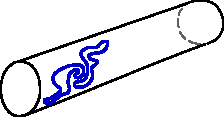
\includegraphics[width=\unitlength]{A27a-pipeSymms}}%
    \put(0.61583231,0.13683004){\color[rgb]{0,0,0}\makebox(0,0)[lb]{\smash{$z$}}}%
    \put(0.00611823,0.27217453){\color[rgb]{0,0,0}\makebox(0,0)[lb]{\smash{$\theta$}}}%
  \end{picture}%
(b)
  \begin{picture}(1,0.52454249)%
    \put(0,0){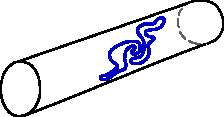
\includegraphics[width=\unitlength]{A27b-pipeSymms}}%
    \put(0.61583231,0.13683004){\color[rgb]{0,0,0}\makebox(0,0)[lb]{\smash{$z$}}}%
    \put(0.00611823,0.27217453){\color[rgb]{0,0,0}\makebox(0,0)[lb]{\smash{$\theta$}}}%
  \end{picture}%
\\
(c)
  \begin{picture}(1,0.52454249)%
    \put(0,0){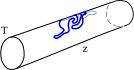
\includegraphics[width=\unitlength]{A27c-pipeSymms}}%
    \put(0.61583231,0.13683004){\color[rgb]{0,0,0}\makebox(0,0)[lb]{\smash{$z$}}}%
    \put(0.00611823,0.27217453){\color[rgb]{0,0,0}\makebox(0,0)[lb]{\smash{$\theta$}}}%
  \end{picture}%
(d)
  \begin{picture}(1,0.52454249)%
    \put(0,0){
\includegraphics[width=\unitlength]{A27d-pipeSymms}}%
    \put(0.61583231,0.13683004){\color[rgb]{0,0,0}\makebox(0,0)[lb]{\smash{$z$}}}%
    \put(0.00611823,0.27217453){\color[rgb]{0,0,0}\makebox(0,0)[lb]{\smash{$\theta$}}}%
  \end{picture}%
 \end{center}
 \caption[$\On{2}_\theta \times \SOn{2}_z$ symmetry of flow in a stream-wise
          periodic pipe]{
A fluid state in a stream-wise periodic pipe translated or rotated is
also a solution. In particular, a \rpo\ $p$ is a state of the fluid
 (a)
that reemerges
 (b)
period $\period{}$ later, translated by downstream shift $\shift$
(in contrast to a \reqv, a constant shape that travels
downstream with constant {\phaseVel} $\velRel$); such solutions are
stream-wise $\SOn{2}_z$ equivariant; or
 (c)
period $\period{}$ later, translated by downstream shift $\shift$ and
rotated azimuthaly by $\gSpace_p$; $\SOn{2}_{\theta} \times \SOn{2}_z$
equivariant; or
 (d)
period $\period{}$ later, reflected and rotated azimuthaly by
$\gSpace$; $\On{2}_{\theta}$ equivariant
(from \wwwcb{}).
 }\label{fig:A27-pipeSymms}
 \end{figure}
%% A27*-pipeSymms.* %%%%%%%%%%%%%%%%%%%%%%%%%%%%%%%%%%%%%%%%%%%%%%%%%%%%%%%

What is a symmetry? A visualization of fluid dynamics of a pipe flow,
\reffig{fig:A27-pipeSymms}, affords an intuitive illustration.
A stream-wise periodic pipe flow under azimuthal rotations and stream-wise
translation (those also become \SOn{2} rotations in a numerical stream-wise
periodic pipe).

Each \SOn{2} group orbit is topologically a circle, but it traces out a
complicated \statesp\ curve composed of many Fourier modes nonlinearly
coupled by turbulent dynamics and thus of comparable magnitudes. Together
the two \SOn{2} sweep out contorted and hard to visualize $T^2$ tori (see
\refref{ACHKW11}), but we shall illustrate here the key ideas by a much
simpler example, the $\SOn{2}$-equivariant Gibbon and
McGuinness\rf{GibMcCLE82,FowlerCLE82} \cLe\ of geophysics and laser
physics,
\bea
	\dot{x}_1 &=& -\sigma x_1 + \sigma y_1
        \,,\qquad
	\dot{x}_2 \,=\, -\sigma x_2 + \sigma y_2
        \continue
	\dot{y}_1 &=& (\RerCLor-z) x_1 - \ImrCLor x_2 -y_1-e y_2 \continue
	\dot{y}_2 &=& \ImrCLor x_1 + (\RerCLor-z) x_2 + e y_1- y_2\continue
	\dot{z} \; &=& -b z + x_1 y_1 + x_2 y_2
    \,.
\label{eq:CLeR}
\eea
Here the parameters are set to Siminos values $\RerCLor=28,\,
\ImrCLor=0,\, b=8/3,\, \sigma=10,\, e= 1/10$. (For the background and an
in-depth investigation of the model  see \refrefs{SiminosThesis,SiCvi10}.)

\begin{figure}
  	\begin{center}
  	\setlength{\unitlength}{0.20\textwidth}
  (a)
  	\begin{picture}(1,1.07802818)%
    	\put(0,0){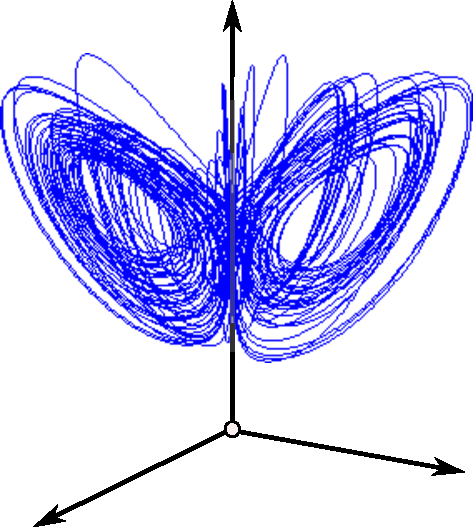
\includegraphics[width=\unitlength]{CLWattractor}}%
    	\put(0.55152995,1.0139628){\color[rgb]{0,0,0}\makebox(0,0)[lb]{\smash{$z$}}}%
    	\put(0.05573445,0.0739776){\color[rgb]{0,0,0}\makebox(0,0)[lb]{\smash{$x_1$}}}%
    	\put(0.90013492,0.16491708){\color[rgb]{0,0,0}\makebox(0,0)[lb]{\smash{$x_2$}}}%
  	\end{picture}%	
  (b)
  	\begin{picture}(1,1.06440474)%
    	\put(0,0){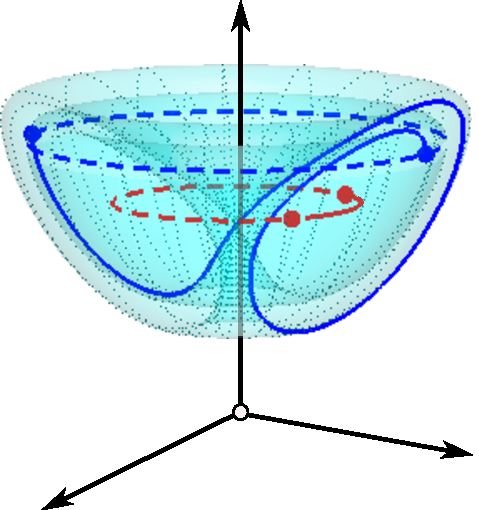
\includegraphics[width=\unitlength]{CLEWurst01}}%
   		\put(0.55961552,1.00214901){\color[rgb]{0,0,0}\makebox(0,0)[lb]{\smash{$z$}}}%
   		\put(0.07008555,0.07304272){\color[rgb]{0,0,0}\makebox(0,0)[lb]{\smash{$x_1$}}}%
    	\put(0.90381504,0.16283301){\color[rgb]{0,0,0}\makebox(0,0)[lb]{\smash{$x_2$}}}%
  	\end{picture}	
    \end{center}
  \caption
  [\CLf: $\cycle{01}$ {\rpo} group orbit]{
  (a)
  The strange attractor of \cLf.
  (b)
  The initial \reqv\ $\REQV{}{1}$ point is shown by the red dot, and its
  group orbit / trajectory by the dashed red line. One period of the
  $\cycle{01}$ {\rpo} is shown by the solid blue line. The group orbit of
  its (arbitrary) starting point is shown by the dashed blue line: after
  one period the trajectory has returned to the group orbit but with a
  different phase. The wurst, \ie, the group orbit of the $\cycle{01}$
  trajectory (dark blue) is shown by the cyan surface. Trajectory of the
  further 15 repeats of $\cycle{01}$ (faint dotted lines) traces out this
  torus; in that time the slowly drifting \reqv\ $\REQV{}{1}$ has
  advanced to the next red dot (red line).
  }
\label{fig:CLf01group}
\end{figure}

The strange attractor of the \cLf\ is shown in
\reffig{fig:CLf01group}\,(a). It's a mess. Why? The problem of dynamics
in presence of symmetry can perhaps be understood this way: dissipative
flows settle into solutions with low friction, and as drifting is
energetically cheap, rather than do work, solutions tend to drift along
non-shape-changing symmetry directions which burn no energy.
    \KC{2012-04-13}{I do not understand the paragraph}
    \PC{2012-04-12 remember to throw away cLe-fullDB.png }

A continuous symmetry leads to drifting invariant solutions.
A {\em \reqv} (traveling wave, rotational wave, ...) is a trajectory
whose velocity field lies within the group tangent space,
\(
\vel(\ssp) = c \cdot \groupTan(\ssp)
\) %\label{phaseVel}
with a constant {\phaseVel} $c$, and whose time evolution is thus
confined to the group orbit; think of an unchanging body carried by a
stream. A {\em \rpo} $\pS_p$ is a trajectory which exactly recurs
\beq
\ssp(\zeit) = \LieEl_p \, \ssp(\zeit + \period{p} )
    \,,\qquad
\ssp(\zeit) \in \pS_p
\ee{RPOrelper1}
after a fixed {relative period} $\period{p}$, but shifted by a fixed
group action ${\LieEl}$ that maps the endpoint $\ssp (\period{}) $ back
into the initial point cycle point $\ssp (0) $; think of a dancer moving
across the stage through a set of motions and then striking the initial
pose, or study the pipe flow sketches \reffig{fig:A27-pipeSymms}.

As the $\SOn{2}$ transformations act on the \cLf\ only through the
simplest, $m=1$ Fourier mode, here all group orbits are circles, and appear
elliptical in most $d=5 \to 3$~dimensions projections. Nevertheless, even
the wurst traced out by the very simplest, short \rpo\ $\cycle{01}$ shown
in \reffig{fig:CLf01group}\,(b) is not so easy to get one's head around:
you are looking at a 3\dmn\ projection of a \emph{torus} embedded in 5
dimensions.

%%%%%%%%%%%%%%%%%%%%%%%%%%%%%%%%%%%%%%%%%%%%%%%%%
% 2011-09-09, 2012-03-30 Predrag: add BeThMovFr to
%            continuous.tex overheads, and ChaosBook
% replace A27movFrame*.* everywhere
\begin{figure}
 \begin{center}
  \setlength{\unitlength}{0.20\textwidth}
  %% \unitlength = units used in the Picture Environment
(a)~~
  \begin{picture}(1,0.98655417)%
    \put(0,0){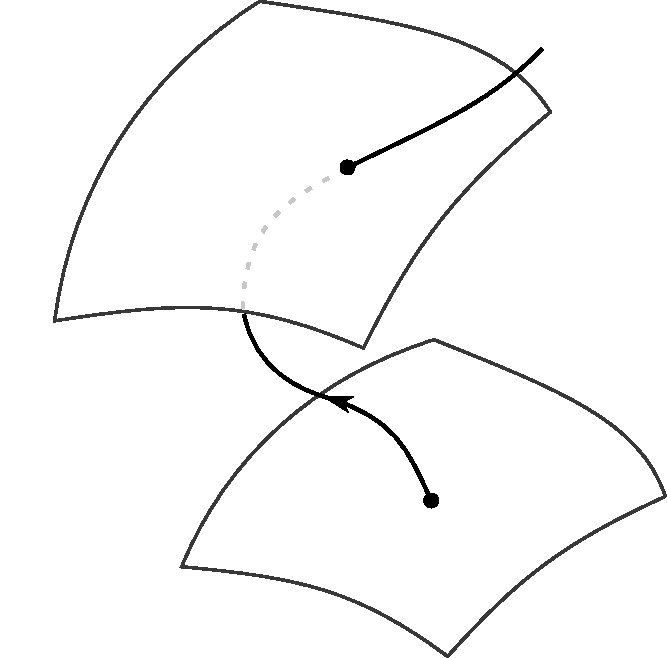
\includegraphics[width=\unitlength]{BeThTrajTeX}}%
    \put(0.35976094,0.91875614){\color[rgb]{0,0,0}\rotatebox{-31.32889204}{\makebox(0,0)[lb]{\smash{$\pS_{\ssp(\zeit)}$}}}}%
        \put(0.60333631,0.42274457){\color[rgb]{0,0,0}\rotatebox{-40.8073288}{\makebox(0,0)[lb]{\smash{$\pS_{\ssp(0)}$}}}}%
    \put(0.66001383,0.16959019){\color[rgb]{0,0,0}\rotatebox{0.0313674}{\makebox(0,0)[lb]{\smash{$\ssp(0)$}}}}%
    \put(0.5058276,0.64524238){\color[rgb]{0,0,0}\rotatebox{0.0313674}{\makebox(0,0)[lb]{\smash{$\ssp(\zeit)$}}}}%
    \put(0.13110825,0.05766516){\color[rgb]{0,0,0}\rotatebox{0.11031334}{\makebox(0,0)[lb]{\smash{$\pS$}}}}%
  \end{picture}%
~~(b)
  \begin{picture}(1,0.98655417)%
    \put(0,0){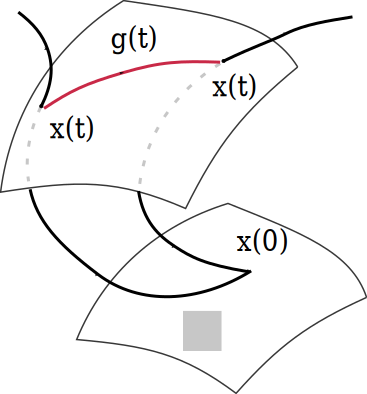
\includegraphics[width=\unitlength]{BeThMovFr}}%
    \put(0.20559239,0.64023845){\color[rgb]{0,0,0}\rotatebox{0.0313674}{\makebox(0,0)[lb]{\smash{$\ssp(\zeit)$}}}}%
    \put(0.67382401,0.35781161){\color[rgb]{0,0,0}\rotatebox{0.0313674}{\makebox(0,0)[lb]{\smash{$\ssp(0)$}}}}%
    \put(0.61221026,0.74589514){\color[rgb]{0,0,0}\rotatebox{0.0313674}{\makebox(0,0)[lb]{\smash{$\sspRed(\zeit)$}}}}%
    \put(0.35760559,0.8662057){\color[rgb]{0,0,0}\rotatebox{0.0313674}{\makebox(0,0)[lb]{\smash{$\LieEl(\zeit)$}}}}%
  \end{picture}%
 \end{center}
  \caption{\label{fig:BeThMovFr}
(a)
The group orbit $\pS_{\ssp(0)}$ of \statesp\ point $\ssp(0)$, and the
group orbit $\pS_{\ssp(\zeit)}$ reached by the trajectory $\ssp(\zeit)$ time $t$
later.
(b)
The two physically equivalent flows
$\ssp(\zeit)=\LieEl(\zeit)\,\sspRed(\zeit)$ are related by, in general,
an arbitrary, time dependent {\em moving frame} transformation
$\LieEl(\zeit)$.
(from \wwwcb{}).
  }
\end{figure}
%%%%%%%%%%%%%%%%%%%%%%%%%%%%%%%%%%%%%%%%%%%%%%%%%%

Evolution in time decomposes the \statesp\ into spaghetti of 1\dmn\
trajectories $\ssp(\zeit)$, each determined by a single point $\ssp(0)$
on it. A section of codimension 1 `quotients' the continuous time
parameter $\zeit$, but for unstable trajectories one really needs a set
of short-time recurrence separated points $\{\sspRed_n\} =
\{\ssp(\zeit_n)\}$ to capture a chaotic flow.

Symmetries stratify the \statesp\ into an onion, each layer a group orbit
(\reffig{fig:BeThMovFr}). We are free to replace a given flow
$\ssp(\zeit)$ by another, physically equivalent flow
$\ssp(\zeit)=\LieEl(\zeit)\,\sspRed(\zeit)$ by any, in general time
dependent {\em moving frame} transformation $\LieEl(\zeit)$. For example,
to film our dancer we can mount the camera on a cart moving alongside
her. So, in presence of continuous symmetries, there are two kinds of
change in time: a dancer, continuously changing shapes, or a drifter, merely
shuffling along the easy, shape non-changing directions. We will presently
banish the drifters, and just enjoy the dance.

% equilibria.tex
% Predrag extracted from newton.tex 		jul  3 2006
% Predrag					jun 20 2006
% Vaggelis					may 20 2006
% $Author$ $Date$

\section{\Eqva} % of the \KSe}
\label{sec:stks}

% Predrag                                       05dec2004
% Lan                                           25nov2004
% from Lan thesis                                8jun2004

\noindent
\Eqva\  (or the steady solutions)
are the simplest invariant sets in
the phase space. They,  and 
the connections between them form the
coarsest geometrical framework for organizing
phase space orbits. %\rf{ksgreene88}.

The \eqv\ condition $u_t=0$ for the {\KSe} PDE \refeq{ks-L} 
is the ODE
\[
(u^2)_x-u_{xx}- u_{xxxx}=0 
% \,.
\]
which can be analyzed as a dynamical system in its own right.
Integrating once we get
\beq
u^2-u_x- u_{xxx}=c 
\,,
\label{eq:stdks}
\eeq
where $c$ is an integration constant 
whose value strongly influences the nature of
the solutions. %of \refeq{eq:stdks}. 
Written as a 3-dimensional dynamical system
with spatial coordinate $x$ playing the role of ``time'',
%\refeq{eq:stdks} 
this is a volume preserving flow
\beq
u_x = v \,,\qquad
v_x = w \,,\qquad
w_x = u^2-v-c \,,
  \label{eq:3dks}
\eeq
with the ``time'' reversal symmetry, 
\[
x \to -x,\quad u \to -u, \quad v \to v, \quad w \to -w \,.
\]
 From \refeq{eq:3dks} we see that
\[
(u+w)_x=u^2-c \,.
\]
If $c<0$, $u+w$ increases without bound with $x \to \infty$,
and every solution escapes to infinity.
If $c=0$, the origin $(0,0,0)$ is the
only bounded solution. 

For $c>0$ there is much
$c$-dependent interesting dynamics, with
complicated fractal sets of bounded solutions.
The sets of the solutions of the \eqv\ condition 
\refeq{eq:3dks} are themselves in turn organized by the  
{\eqva} of the \eqv\ condition, and 
the connections between them.
    For $c>0$ the \eqv\ points of \refeq{eq:3dks} are
$c_{+}=(\sqrt{c},0,0)$ and $c_{-}=(-\sqrt{c},0,0)$.
Linearization of the flow around
$c_{+}$ yields 
stability eigenvalues 
\beq
 [2\lambda \,, -\lambda \pm i \theta ] 
\,,\qquad
\lambda=\frac{1}{\sqrt{3}}\sinh \phi
\,,\qquad
\theta=\cosh \phi \, ,
\label{eqvEqvEigV}
\eeq
and $\phi$ fixed by $\sinh 3\phi=3\sqrt{3c}$. 
Hence $c_{+}$ has a {1-dimensional}
unstable manifold and a 2-dimensional
stable manifold along which solutions spiral 
in. 
By the $x \to -x$ ``time reversal'' symmetry, the 
invariant manifolds of $c_{-}$ 
have reversed stability properties.

\PublicPrivate{%
		}{% switch to Private:

\subsection{Heteroclinic and homoclinic connections}
%
% from \Chapter{KS}{12Jun2004}{Steady solutions of KS equation}
% Lan                                            8Jun2004

\PC{either drop this, or credit \refref{Lan:Thesis,LanCvi06}
    if we need it
   }
\KSe\ \refeq{eq:stdks} has an exact heteroclinic solution
\beq
u=a_1 \tanh(kx)+a_2 \tanh^3(kx)
\label{eq:ksexa} 
\,,
\eeq
for the specific value $c=-\frac{30k^2}{19}(304k^4-40k^2+1)$ where 
\[
a_1=60k^3-\frac{30k}{19}\,,\;a_2=-60k^3
	\,,\qquad
k^2=11/76 \mbox{ or } 
k^2=-1/76
\,.
\]
When $k^2=-1/76$, the hyperbolic tangent becomes ordinary tangent and there are poles on
the real axis. Near the singularity, $u$ blows up as
\[
u(x) \approx \frac{-60}{(x-x_0)^3}\,,\; x \to x_0 
\,.
\]
All the blow-up solutions possess singularities of the same type\rf{ksham95}.
% In general, the existence and structure of connections depend on parameter
% $c$ in a complicated way.
		}% end \PublicPrivate

\subsection{\KSe\ on a periodic domain}
% However, we do not need to explore the fractal set of the 
% \KS\ {\eqva} for infinite size system here;
For a fixed system size 
$L$ with periodic boundary condition, the only surviving {\eqva}  are
those with periodicity $L$.
They satisfy 
the \eqv\ condition for \refeq{expan}
\PC{\rf{ksgreene88} to remarks}
\beq
(k/\tilde{L})^2\left( 1 - (k/\tilde{L})^2  \right)b_k 
	 + i (k/\tilde{L}) \sum_{m=-\infty}^{+\infty} b_m b_{k-m} = 0
\,.
\label{eq:stfks}
\eeq 
% We have proved in \refsect{sec:kspr} that 
Periods of spatially periodic {\eqva} are multiples of $\tildeL$.
Every time $\tilde{L}$ crosses an integer value  $\tilde{L}=n$,
$n$-cell states
are generated through pitchfork bifurcations. 
In the full phase space they
form an invariant circle due to the translational invariance of \refeq{ks-L}. 
% In the antisymmetric subspace considered here, they corresponds to two points,
% half-period translates of each other of the form
% \[
% u(x,t)=-2\sum_k b_{kn}\sin (knx) \,,
% \]
% where $b_{kn} \in \mathbb{R}$.
% % By rescaling $u,x$ and $\nu$, the $n$-cell states transform to each other.

%      With the increase of $L$ these periodic solutions 
% may bifurcate into more complicated ones.
For any fixed period $L$
%, however, 
the number 
of spatially periodic solutions is finite up to a spatial translation.
This observation can be heuristically motivated as follows. 
% \PC{this argument keeps worrying me: there are lots of solutions, like
% $u=0$, that are {\eqva}, but isolated -
% they are noplace near asymptotic dynamics.
% Do they belong to the invariant manifold?
%    }
% Equilibria are solutions valid for all times, and are thus points
% on the finite-dimensional compact inertial manifold\rf{infdymnon}.
Finite dimensionality of the inertial manifold
bounds the size of Fourier components of all solutions.
% This
% compact inertial manifold and the dynamics on it can be 
% described by analytic functions of a finite number of Fourier modes.
\PC{explain the theory; say that in practice it is useless}
On a finite-dimensional compact manifold,
an analytic function can only have a finite number
of zeros. So, the {\eqva}, {\em i.e.}
the zeros of a smooth velocity field on
the inertial manifold, are finitely many.
% The number of {\eqva} increases exponentially with $L$,
% \PC{give reference for ``exponential growth''}
% for infinite system size $L \to \infty$,
% there are infinitely many {\eqva}. 
% \PC{is there a reference where this is explained?}

For a sufficiently small $L$ 
the number of {\eqva} is small,
mostly
concentrated on the low wave number end of the Fourier spectrum.
These solutions may
be obtained by solving the truncated versions of \refeq{eq:stfks}. 
% Understanding the structure of these solutions, requires a study
% of the full phase space of the 3-dimensional dynamical system \refeq{eq:3dks},
% not attempted here.

% Locally coherent structures are observed for arbitrary system size,
% see \reffig{f:flameFlut}~(b). %\reffig{f:ksev}.


% \index{Kuramoto-Sivashinsky \eqva\}
% \index{equilibria!Kuramoto-Sivashinsky}



% \PC{say somewhere: ``
% The task of the theory is to describe this spatio-temporal
% turbulence and yield quantitative predictions for its measurable
% consequences.
%    ''}


In a periodic box of size $L$
both \eqva\ and \reqva\ are  periodic solutions 
embedded in 3-$d$ space \refeq{eq:3dks}, 
conveniently represented as loops in 
$(u,v,w)$ space whose topology is controled by
``\eqva\ of \eqva\'' stable-unstable manifold structure of
\refeq{eqvEqvEigV}.
In this representation the continuous translation symmetry
is automatic - a rotation in the $[0,L]$ periodic domain only
moves the points along the loop. For an \eqv\ the points
are stationary in time; for \reqv\ they move in time, but in
either case, the loop remains invariant.
So we do not have the problem that we encounter in the Fourier 
represenation, where from the frame of one of the \eqva\
the rest trace out circles under the action of continuous symmetry 
translations.

The $c$ integration constant also means something, we are not quite sure
what.


Perhaps there is some way of plotting the unstable manifolds too. If
there is only one unstable direction (in the full Fourier space
representation), the corresponding eigenvector is a unique loop function
$h[s] =  h(u(s),v(s),w(s))$ in the $(u,v,w)$ space, and the unstable manifold
$U$ is swept out by evolving in time the perturbed loop 
$L[s] + \delta h[s] =  L(u(s),v(s),w(s)) + \delta h(u,v,w)$
$\to$ $L[s,t]$.
Complex eigenvector defined unstable manifold plane seems
harder to visualize;  It would be interesting
to look at heteroclinic connections in the $(u,v,w)$ space, as
behavior of higher-frequency modes in Fourier reps is a bit
hard to get used to.



\section{Why does a flame front flutter?}
\label{s:StabEqui}
%%
% Predrag           5jun2005
% extracted from \Chapter{stability}{ 2apr2005}
% Predrag                  14/3-95
% taken from ks.tex

% \index{local!stability}
% \index{linear!stability}
% \index{stability!linear}
% \index{equilibrium!point}

We start by considering the case where
$a_\stagn$ is an \eqv\ point \refeq{EquilPoint}. 
Expanding around the \eqv\ point $a_\stagn$,
and using the fact that the matrix
${\bf \Mvar}={\bf \Mvar}(a_\stagn)$
% , its matrix of its stability exponents
in \refeq{die}
% local expansion rate
is constant, 
we can apply the simple formula \refeq{eqPointStab} also to the 
{\jacobianM}
of an \eqv\ point of a PDE, 
\[
 \jMps^t(a_\stagn) = e^{{\bf \Mvar} t}
    \,\qquad
 {\bf \Mvar}={\bf \Mvar}(a_\stagn)
\,.
\]

The \KS\ flat flame front $u(x,t)=0$ is an 
\eqv\ point of \refeq{ks}. The matrix of variations
\refeq{DerMatrix}
follows from \refeq{expan}
% \index{Kuramoto-Sivashinsky system}
\beq
{\Mvar}_{kj}(a) ={\pde v_k(a)\over \pde a_j  }
=((k/\tilde{L})^2- (k/\tilde{L})^4)\delta_{kj} - 2(k/\tilde{L}) a_{k-j}
\,.
\ee{expanMvar}
For the $u(x,t)=0$ \eqv\  solution the matrix of variations
is diagonal, and -- as in \refeq{EqDyn164} -- so is the {\jacobianM}
$
\jMps^t_{kj}(0) = \delta_{kj} e^{((k/\tilde{L})^2- (k/\tilde{L})^4)t}
\,.
$

For $\tilde{L} < 1$,  $u(x,t)=0$ is the globally attractive stable 
{\eqv}.
As the system size $\tilde{L}$  is increased,
the ``flame front'' becomes increasingly unstable and turbulent,
the dynamics goes through a rich sequence of
bifurcations on which we shall not dwell here.
% studied e.g. in \refref{KNS90}. 
% , one quickly finds a
% myriad of unstable periodic solutions whose number
% grows exponentially with period.

The $|k|<??$ 
long wavelength perturbations of the flat-front {\eqv}
are linearly unstable, while all 
$|k|> ??$ short wavelength perturbations are strongly contractive.  
The high $k$ eigenvalues, corresponding to rapid variations of
the flame front, decay so fast that the corresponding eigendirections
are physically irrelevant.
% \index{Lyapunov exponent!{\eqv}}
To illustrate the rapid contraction in the non-leading eigendirections
we plot  in [MAYBE INCLUDE] % \reffig{f:eigenvalues}
the eigenvalues of the \eqv\ in the unstable regime,
for relatively small system size, % low viscosity $\nu$,
and compare them with the
stability eigenvalues of the least unstable cycle for the same 
system size.
% value of $\nu$. 
The \eqv\ solution is very unstable,
in 5 eigendirections,
the least unstable cycle only in one. 
Note that for $k>7$ the rate of contraction
is so strong that higher eigendirections are numerically meaningless for 
either solution; even though the flow is infinite-dimensional, the attracting
set must be rather thin.

While in general
for $\tilde{L}$ sufficiently large
one expects many 
coexisting attractors in the phase space%
%Hyman and Nicolaenko
\rf{HNZks86} ,
in numerical studies most random initial
conditions settle converge to the same chaotic attractor. 

From \refeq{expan} we see that the origin $u(x,t) = 0$
has Fourier modes as the  linear
stability eigenvectors. 
When $|k| \in (0,\tilde{L})$, the corresponding Fourier modes are
unstable.
The most unstable modes has $|k|=\tilde{L}/\sqrt{2}$ and defines the scale of basic building
blocks of the spatiotemporal dynamics of the {\KSe} in large system size limit,
as shown in \refsect{sec:KSnumer}. 


% \noindent
% Consider now the case of initial $a_k$ sufficiently small
% that the bilinear $ a_m a_{k-m}$ terms in \refeq{expan} can
% be neglected. Then we have a set of decoupled linear
% equations for $a_k$ whose solutions are exponentials, at most
% a finite number for  which
% $k^2 > \nu k^4$
% is growing with time, and infinitely many with
% $
% \nu k^4 > k^2
% $
% decaying in time.
% The growth of the unstable long wavelengths (low $|k|$) excites
% the short wavelengths
% through the nonlinear term in \refeq{expan}.  The excitations thus
% transferred are dissipated by the strongly damped short wavelengths,
% and a ``chaotic \eqv\'' can emerge. The very short
% wavelengths $|k| \gg 1 / \sqrt{\nu}$ remain small for all times,
% but the intermediate wavelengths of order $|k| \sim 1 / \sqrt{\nu}$
% play an important role in maintaining the dynamical {\eqv}.
% As the damping parameter decreases, the solutions increasingly take on
% % Burgers type
% shock front
% character poorly represented by the Fourier basis, and many
% higher harmonics may need to be kept
% % \rf{KNS90,GEP}
% in truncations of
% \refeq{expan}.
% 
% 
% Hence, while one may truncate the high modes in the expansion
% \refeq{expan}, care has to be exercised to ensure that no modes
% essential to the dynamics are chopped away. 
% 
Even though our starting point
\refeq{ks}
is an infinite-dimensional dynamical system, the asymptotic dynamics
unfolds on a finite-dimensional attracting manifold, and so we are back on
the familiar territory of \refsect{SecDynFlows}:
the theory of a finite number of ODEs applies to this
infinite-dimensional PDE as well.

    {\bf When is an \eqv\ important?} There are two kinds of roles
{\eqva} play:

{\em ``Hole'' in the natural measure}.
The more unstable eigendirections it has (for example, the
$u=0$ solution), the more unlikely it is  that
an orbit will recur in its neighborhood.

{\em unstable manifold of a ``least unstable''{\eqv}}.
 Asymptotic dynamics
spends  a large fraction of time in
neighborhoods of a few  {\eqva} with
only a few unstable eigendirections.


\underline{\KS\ system, truncations.}{
We describe here our criterion for reliable
truncations of the infinite ladder of 
ordinary differential equations (\ref{expan}).

Adding an extra dimension to a truncation of the system (\ref{expan})
introduces a small
perturbation, and this can (and often will) 
throw the system into a totally different asymptotic state. 
A  chaotic attractor for $N=15$ can become a period three 
window for $N=16$, and so on. 
If we compute, for example, the Lyapunov exponent
$\Lyap(\nu,N)$ for the strange attractor of the 
system (\ref{expan}), there is no reason to 
expect $\Lyap(\nu,N)$ to smoothly converge to the limit  
value $\Lyap(\nu,\infty)$ as $N \rightarrow \infty$. 
The situation is different in the periodic windows, 
where the system is structurally stable, and it makes sense to compute 
 Lyapunov exponents, escape rates, etc. for the 
{\em repeller}, \ie, the closure of the set of all 
{\em unstable} periodic orbits. 
Here the power of cycle expansions comes in: 
to compute quantities on the repeller by direct averaging methods is 
generally more difficult, because the motion quickly collapses to the 
stable cycle. 
	} %end \remark{Kuramoto-Sivashinsky system, numerical results.}


The problem one faces with high-dimensional flows is 
that their topology is hard to
visualize, and that even with a decent starting guess for a point on
a periodic orbit, methods like the Newton-Raphson method are likely to fail.
Methods that start with initial guesses for a number of points along the
cycle, such as the multipoint shooting method of \refsect{s-MultShoot},
are more robust.
The relaxation  (or variational) methods take this strategy to its
logical extreme,
and start by a guess of not a few points along a periodic orbit,
but a guess of the entire orbit.

At present the theory is in practice applicable only to systems
with a low intrinsic {\em dimension}
-- the minimum number of coordinates necessary to
capture its essential dynamics.
% \index{dimension!intrisic}
% \index{degree of freedom}
If the system is very turbulent
(a description of its long time dynamics requires a space of high
intrinsic dimension) we are out of luck. 
% \index{turbulence}

% \input{chapter/refsPDEs}

%%% end


% newton.tex
%
% Predrag			jun 20 2006
% Vaggelis			may 20 2006
% $Author$ $Date$


% \section{Newton's method for determining \reqva}
% 
%  Our task is to find \reqva\ solutions of \refeq{eq:KS}.
% Although one can easilly see that this problem can be reduced to that of
%  finding periodic orbits of a 4-dimensional ODE, here we prefer to consider our system in phase space and search for solutions of
%  \beq
% 	\dot{b}_k=\dot{c}_k=0\,,
%  \eeq
%  for every $k$. The reason to do this is just getting experience before pursuing the more difficult task of locating POs and RPOs. 
%  Expanding $\dot{b}_k(a)$ and $\dot{c}_k(a)$ around our initial guess $a_o$ and demanding that they satisfy the equilibrium 
%  condition, we get
%  \bea
% 	\dot{b}_k(a) & = & \dot{b}_k(a_o)+\left.\frac{\partial \dot{b}_k}{\partial b_j}\right|_{a_o}\delta b_j + \left.\frac{\partial \dot{b}_k}{\partial c_j}\right|_{a_o}\delta c_j = 0 \continue
% 	\dot{c}_k(a) & = & \dot{c}_k(a_o)+\left.\frac{\partial \dot{c}_k}{\partial b_j}\right|_{a_o}\delta b_j + \left.\frac{\partial \dot{c}_k}{\partial c_j}\right|_{a_o}\delta c_j = 0
%  \eea
%  or in matrix form
%  \beq
%     \left( \begin{array}{cc}
%         \frac{\partial \dot{b}}{\partial b} & \frac{\partial \dot{b}}{\partial c} \\
%         \frac{\partial \dot{c}}{\partial b}	& \frac{\partial \dot{c}}{\partial c}
%      \end{array}
%      \right)_{a_o}
%      \left(\begin{array}{c}
%        \delta b  \\
%        \delta c
%      \end{array}\right)
%      =
%      \left(\begin{array}{c}
%        -\dot{b}(a_o) \\
%        -\dot{c}(a_o)
%      \end{array}\right)\,,
%      \label{eq:NewtonEquil}
% \eeq
% where $\partial{\dot{b}} / \partial{b}$ \etc are $d \times d$ submatrices. Solving this
% system of equations for the corrections $\delta b$ and  $\delta c$ and using the refined solution
% as an initial guess yields  an approximation to the solution of the system.
%  


\subsection{Implementing Newton's method  for RPOs}
\label{sec:NewtRPOs}

The relative periodic condition
\beq
	u(x+d,t+T)=u(x,t) \,
\eeq
translates in Fourier space into
\beq	
	\sum_{k=-\infty}^{+\infty} a_k (t+T) e^{ i k (x+d) / \tildeL} 
		= \sum_{k=-\infty}^{+\infty} a_k (t) e^{ i k x / \tildeL} \,
\eeq
or
\beq
	e^{ik\, d /\tildeL}a_k(t+T)=a_k(t) \,,\ \forall k \in \mathds{Z}\ \ \ \mathrm{(no\ summation)}.
	\label{eq:RPOcondition}
\eeq
We see that a relative periodic orbit returns after time $T$ to a point in 
phase space with components $a_k(t+T)$ rotated in the complex plane by an 
angle $-k\, d /\tildeL$ with respect to $a_k(t)$. In matrix notation, we write \refeq{eq:RPOcondition} as
\beq
	\mathbf{g}(d)  a(t+T)=a(t)\,,
	\label{eq:RPO}
\eeq
where we have defined
\beq
	\mathbf{g}(d) \equiv Diag[e^{ik\, d/\tildeL}]\,.
\eeq
%We notice that $R(\kappa)$ is not a rotation operator..

% Consider an initial guess $a'$ for a point on a relative periodic orbit and assume that it lies on
% a \Poincare section $\mathcal{P}$ at $t=0$. Suppose that $\mathcal{P}$ is a hyperplane in
% $\mathds{R}^{2d}$. The flow $f^t$ defined by \refeq{eq:Fcoef} transports 
% this point after time $T'$ into $a'(T')=f^{T'}(a')$. Suppose that this point is such that $R(\kappa')f^{T'}(a')$
% is a point on $\mathcal{P}$. Consider next a point $a$ lying on $\mathcal{P}$ and in the neighborhood of $a'$,
% thus satisfying
% \beq
% 	q \cdot (a'-a) = 0\,,
% 	\label{eq:cond a}
% \eeq
% with $q$ a vector normal to $\mathcal{P}$. Point $a$ will be finally identified with the improved 
% approximation of a point on the periodic orbit.
% The flow transports $a$ to $f^{T'}(a)$, but now $R(\kappa')f^{T'}(a)$ is not in general on $\mathcal{P}$.
% Moreover we would like to have the freedom to adjust the guesses for $T'$ and $\kappa'$ into new values
% $T=T'+\Delta T$ and $\kappa=\kappa'+\Delta \kappa$ to improve their accuracy. 
% Let as consider such slightly different values $T$ and $\kappa$ such that $R(\kappa)f^{T}(a)$ lies on 
% $\mathcal{P}$. Then we have the condition
% \beq
% 	q \cdot(R(\kappa')f^{T'}(a')-R(\kappa)f^{T}(a)) = 0\,.
% 	\label{eq:cond Rf(a)}
% \eeq 

Starting with an initial guess $a$ for a point on a \rpo\ we use Newton's method to find an improved approximation to the true solution $a^*$ of condition  \refeq{eq:RPO}:
\beq
	a^*=\mathbf{g}(d^*)  f^{T^*}(a^*)\,,
	\label{eq:RPOcond}
\eeq
with period $T^*$ and shift $d^*$. Let $T$ and $d$ be our guess period and shift, respectively. 
Taylor expanding $\mathbf{g}(d^*)  f^{T^*}(a^*)$ around $a$ to linear order in the small quantities 
$\delta a=a^*-a$, $\delta T=T^*-T$ and $\delta d=d^*-d$, we get
% \bea
% 	f^{T}(a)& \simeq & f^{T}(a')+\J^T(a') \Delta a \label{eq:fTaylorl1} \\ 
% 		& \simeq & f^{T'}(a') + v \Delta T + \J^{T'}(a') \Delta a \label{eq:fTaylorl2} \,, 
% \eea
% where $v$ is evaluated at $f^{T'}(a')$. Here $\J^t(x)$ is the Jacobian matrix, defined for a general flow through
% \beq
%    	J^t_{ij}(x_o)=\left.\frac{\partial x_i(t)}{\partial x_j}\right|_{x=x_0}\,.
% \eeq
% The Jacobian matrix is obtained by integrating the equation:
% \beq
%    	\dot{\mathbf{J}}^t=\mathbf{A J}^t \, ,
% 	\label{eq:Adef}
% \eeq
% subject to the initial condition:
% \beq
%    	\mathbf{J}^0=\mathbf{1} \, ,
% \eeq
% Here $\mathbf{A}$ is the matrix of variations defined as:
% \beq
% 	A_{kj}=\frac{\partial \dot{x}_k}{\partial x_j}\,.
% \eeq
% 
% In passing from \refeq{eq:fTaylorl1} to \refeq{eq:fTaylorl2} we have used the multiplicative 
% structure of the Jacobian, $\mathbf{J}^{T'+\delta T}(a')=\mathbf{J}^{\delta T}(f^{T'}(a'))\mathbf{J}^{T'}(a')$, 
% noticed that $\mathbf{J}^{\delta T}(f^{T'}(a'))=e^{\mathbf{A}\delta T}=\mathbf{1}+\mathbf{A}\delta T+\ldots$ 
% and dropped second order terms in the small quantities.
% 
% On the other hand, we have
% \bea
% 	R(\kappa'+\Delta\kappa) & = & R(\kappa')R(\Delta\kappa) \continue
% 				& \simeq & R(\kappa')(\mathbf{1}+iDiag[k]\Delta\kappa/\tildeL)\,.
% 	\label{eq:TaylorR}	
% \eea
% 
% Substituting \refeq{eq:fTaylorl2},\refeq{eq:TaylorR} into \refeq{eq:RPOcond} and keeping only first
% order terms in the small quantities, we get
% \beq
% 	a+\delta a \simeq \mathbf{g}(d)  f^{T}(a) + \mathbf{D[g]}(\mathbf{g}(d) f^{T}(a))\delta d
% 				+ \mathbf{g} (d)v(f^{T}(a)) \delta T + \mathbf{g}(d) \J^{T}(a) \delta a\,,
% \eeq
% or
\beq
	\left(\mathbf{1}-\mathbf{g}(d)\J^{T}(a)\right) \delta a - \mathbf{g}(d)v(f^{T}(a)) \delta T 
							- \mathbf{D[g]}(\mathbf{g}(d)f^{T}(a))\delta d  
					\,\simeq\, \mathbf{g}(d)f^{T}(a)-a\,,
	\label{eq:NewtonBasicCond}			
\eeq
where $D[g]_{kj}=\frac{ik}{\tildeL}\delta_{kj}$. The matrix $\mathbf{g}(d)\J^{T}(a)$ has two unit eigenvalues in 
the limit $a\rightarrow a^*$, one associated with the invariance along the direction of the flow and the other with the
translational invariance of the system. Thus \refeq{eq:NewtonBasicCond} needs to be augmented by two conditions to
eliminate the indeterminacy introduced by the (close to) zero eigenvalues of $\mathbf{1}-\mathbf{g}(d)\J^{T}(a)$. Following 
\refref{ViswanathPC06} we choose the conditions 
\bea
	v(a)\cdot\delta a & = & 0 \label{eq:NewtonAux1} \,\\
	(\mathbf{D[g]}a)\cdot \delta a & = & 0 \label{eq:NewtonAux2}\,.
\eea
The requirement imposed by \refeqs{eq:NewtonAux1}{eq:NewtonAux2}\ on the solution vector $\delta a$ of \refeq{eq:NewtonBasicCond} 
is that it vanishes along the directions of the flow and of infinitesimal translation of the initial condition.

Equations \refeq{eq:NewtonBasicCond} and \refeqs{eq:NewtonAux1}{eq:NewtonAux2}
can be compactly represented in a single matrix equation:
\beq
    \left( \begin{array}{ccc}
       \mathbf{1}-\mathbf{g}(d)\mathbf{J}^{T}(a) 	& -\mathbf{g}(d)v(f^{T}(a))	  & -\mathbf{D[g]}(\mathbf{g}(d)f^{T}(a))  \\
        v(a)^{\dagger}			& 0  	& 0 	\\
        (\mathbf{D[g]}a)^\dagger	& 0 	& 0 
     \end{array}
     \right)
     \left(\begin{array}{c}
       \delta a \\
       \delta T \\
       \delta d
     \end{array}\right)
     =
     \left(\begin{array}{c}
       \mathbf{g}(d)f^{T}(a)-a \\
       0     \\
       0
     \end{array}\right)\,.
     \label{eq:NewtonScheme}
\eeq
where $v^\dagger$ denotes the adjoint of $v$. 

\JFG{Back around \ref{expan} in fourier.tex you mentioned you set the 
coefficients to purely imaginary values $i a_k$ and fixed $a_{-k}= -
a_k$ to assure real-valuedness and to isolate antisymmetric solutions. 
This eliminates continuous translation symmetries. Presumably in this
section, since you're looking for RPOs, this is relaxed. Do you then
enforce real-valuedness in your Newton-descent via the constraint
$a_{-k} = a^*{k}$ (the conjugates that then appear in the equations
are nondifferentiable which is a big pain) or do you let the solutions
go complex and then choose the real part at the end? The cost of that
is that the dimension of your search space is twice as big as it needs 
to be. That's an unacceptable cost in fluids; perhaps in KS it's not. 
In any case, I think you should (1) either clarify that you're no 
longer working in the antisymmetric subspace or eliminate its mention 
earlier, and (2) explain how you ultimately arrive at real-valued 
solutions.}

        \Preliminary{
% variational.tex
%
% Predrag created file				jul 9 2006
% $Author$ $Date$


\section{\descent}


%%%%%%%%%%%%%%%%%%%%%%%%%%%%%%%%%%%%%%%%%%%%%%%%%%%%%%%%%%%%%%%%
\begin{figure}[t] %[h]
\centering
(c) 
\includegraphics[width=2.5cm]{figs/path.eps}
\hspace{0.1in}
(b) 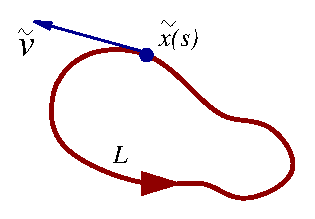
\includegraphics[width=3.5cm]{figs/loop.eps}
\hspace{0.1in}
(c) 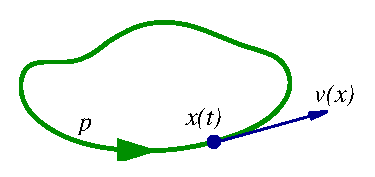
\includegraphics[width=4.0cm]{figs/porbit.eps}
\caption{
 (a) A continuous path; (b) a loop $\Loop$ with its tangent velocity vector $\lVeloc$;
 (c) a periodic orbit $p$ defined by the vector field $\pVeloc(\pSpace)$.
        }
\label{f:loops}
\end{figure}
%%%%%%%%%%%%%%%%%%%%%%%%%%%%%%%%%%%%%%%%%%%%%%%%%%%%%%%%%%%%%%%%%%

    In order to set the notation, we shall distinguish between (see \reffig{f:loops}):

\medskip
\noindent
 {\bf closed path:}
 any closed (not necessarily differentiable) continuous curve 
$J \subset \pS$.

\medskip
\noindent
{\bf loop:}
 a smooth, differentiable closed curve $\lSpace(s)\in \Loop \subset 
\pS$, 
parametrized by $s \in [0,2\pi]$ with $\lSpace(s)=\lSpace(s+2\pi)$, with the
magnitude of the loop tangent vector fixed by 
the (so far arbitrary) parametrization of the loop,
\[
\lVeloc(\lSpace)=\frac{d \lSpace}{ds}\,, \quad \lSpace=\lSpace(s) \in \Loop
\,.
\]   
{\bf annulus:} 
 a smooth, differentiable surface $\lSpace(s,\tau)\in \Loop(\tau)$ swept by a 
family of loops $\Loop(\tau)$, by integration along a fictitious time flow
(see \reffig{f:velocField}~(a))
\[
\dot{\lSpace}=\frac{\partial \lSpace}{\partial \tau}
\,.
\]
{\bf periodic orbit:}
 given a smooth vector field $\pVeloc=\pVeloc(\pSpace),\; (\pSpace,\pVeloc) \in {\bf T} \pS$, periodic orbit $\pSpace(t) \in p$ is a solution of
\[
\frac{dx}{dt}=\pVeloc(\pSpace) 
	\,,\quad
	\mbox{ such that } \pSpace(t)=\pSpace(t+\period{p}),
\] 
where $\period{p}$ is the shortest period of $p$.



The strategy
is to minimize an action functional defined on a space of paths $\gamma$ in the
configuration space $\pS$ which satisfy the property
\beq
                               \gamma (t + T ) = g \cdot \gamma (t)                       
\label{McC1desc}
\eeq
for a fixed {\em relative period} $T$ and some fixed diffeomorphism $g$ of $\pS$, 
sometimes referred to as a {\em phase}, that leaves the 
action functional invariant. If $g^k=1$ is of finite order
$k$, then the corresponding orbit is periodic with period $k T$. 


            } %end \Preliminary{
% KS-L22.tex
%
% Predrag created file				jul  9 2006


\section{Small \KS\ $L=22$ system {\rpo s}}

% Davidchack and Crofts
The full space \KS system $L = 22.0$ 
appears to be the smallest $L$ with persistent chaos.  
$L=22$ is a sensible choice because in units of mean wavelength
the size of this small system is about $ \tilde{L}/\sqrt{2}= 2.4758$
2.5 wavelengths, 
so the dynamics is competition between wavenumbers
2 and 3.
Because of the strong contractionin KS we expect at most 10 eigenvalues to be
significant, rest are in the numerical noise. See figure~6 in
\refref{Christiansen:97}.

% Davidchack and Crofts 
We investigate this system in 15 complex Fourier modes
(30-dimensional system of real ODEs) truncation, and recheck the results 
by redoing the calculation with the double number of Fourier modes.
% observe how many digits change. 
The \eqv\ points are accurate to at least to $10^{-11}$. Since
Lapack is also double precision accurate, the accuracy of the first
few eigenvalues is similar, and certainly in
excess of 6 significant digits.
%
All digits stated in tables are significant.

The accuracy that can be reached is of order of
$|a(\period{p},d_p) - a_0| \approx \epsilon \exp(\Lyap_p \period{p})$,
where $\epsilon \approx 10^{-17}$ for double precision,
$\lambda_p$ is the largest Lyapunov exponent, 
and $\period{p}$ the period.  With a good starting guess,
Newton's method
typically reaches that accuracy after 2-3 iterates.


\Eqva\ and \reqva\ of \KSe\ are investigated in Kevrekidis \etal\rf{saddks}. 
Many of the \rpo s can be constructed from segments corresponding to
close approches to some of these equlibria.

\subsection{\Eqva}

Numerically we find \eqva\ of wavenumber $k$ by (when it exists)
by using $sin( k x /\tilde{L})$ as the initial guess for the Newton routine.
The \eqva\ {\nameit}2 and {\nameit}3 found here
essentially lie in the 2nd and 3rd Fourier component complex planes,
respectively, with very
small deformations from higher harmonics.
\RLD{recheck their $a_1$ content}

For $L = 22.0$ there are at least
3 unstable \eqva\ and a pair of unstable \reqva:

\PC{probably make up a table with all these}
Wavenumber 0 \eqv\ {\nameit}0, $u=0$, with multipliers 
(eigenvalues of $\Mvar$):

\PC{these we have analytically, all real.
Enter values here, refer to the equation}

\PC{why is there no wavenumber 1 \eqv\ {\nameit}1?}

Wavenumber 2 \eqv\ {\nameit}2, with multipliers 
\ES{I observe pairs of real eigenvalues,
e.g. -58.3602685 and -58.3602681. As their absolute
value increases they differ even less.
I think it has to do with the linear part being the main
contribution to $\Mvar$ for higher modes, as well as 
with treating real and imaginary components 
as separate variables, which means it will appear twice.
	}
\PC{I think such contracting eigenvalues as -58.3602685 have no meaning.
Even if they are accurate eigenvalues of $\Mvar$,
what use is
$\ExpaEig_{radial} =  e^{\Lyap_p \period{p}} = e^{26\cdot58} = e^{1510}$.
	}

$(\Lyap_i \pm \theta_i)
=(
  0.13903973 \pm i 0.23842023,
  0,
 -0.08402656 \pm i 0.16019413,
 -0.11941393, 
 -0.27112264 \pm i 0.35630716,
 -2.01303043,
 -2.03775342,
 -5.63649418,
\cdots
)$
\PC{need to decide: eigs either appear as complex pairs, or
real pairs, because of complex Fourier coefficients. Should we list
real pairs? Probably best to list them only once.}

These \eqva\ are selfdual under $u(x) \to -u(-x)$ symmetry.

\PC{figures might be in dasbuch/talks/figs/, repository dasbuch}
% Ruslan L Davidchack, 	10 Jul 2006 
Figure steady\_states2.jpg

% Ruslan L Davidchack, 	10 Jul 2006 
2-wave steady state:

$(\Lyap_i \pm \theta_i)=
(
  0.13903972165535 \pm 0.23842023092014i,
  0.00000000345431                    ,
 -0.08402654994820 \pm 0.16019413653788i,
 -0.11941394469356                    ,
 -0.27112264064485 \pm 0.35630715566102i,
)$

% Ruslan L Davidchack, 	10 Jul 2006 
Wavenumber 3 \eqv\ {\nameit}3, with multipliers 

$(\Lyap_i \pm \theta_i)=
(
  0.09334635581866                    ,
  0.09334403319083                    ,
 -0.00000000000000                    ,
 -0.41277453725606                    ,
 -0.61075248808595 \pm 0.37587414026088i,
)$


\underline{Need to trace out}
the unstable manifold plane, like Gibson did for plane Couette.
Compute the 2 expanding eigenvectors of the
\eqv\ {\nameit}2, as well as the 3rd, least contracting direction; then
translate and rotate your Fourier modes into this coordinate frame,
and plot the trajectory there, both in the lab and the mean velocity frame.

Ruslan: % 10 Jul 2006
% 
% 119 KB     "long_orbit.jpg"
%  88 KB     "steady_states1.jpg"
%  84 KB     "steady_states2.jpg"
% 197 KB     "rpos1.jpg"
% ----------------------------------------

For all spatial plots color axis $u \in [-3, 3]$ is the same,
same time units and spatial width $L$.
For the steady states the magnitude of the 2-wave is quite 
a bit smaller than that of the 3-wave.

In steady\_states1.jpg I've plotted the numerical evolution and, since the
traveling wave is very unstable, it disappears after awhile. I've plotted
analytical solution in steady\_states2.jpg, but thought you might want to
have the first one as well.

rpos1.jpg is attached as a sample. 

\subsection{\Reqva}

Numerical solution of the relative equilibrium condition,
transported by travelling wave velocity $c$, 
fixed by the solution for the travelling wave equation:
\[
f_k(u) - i{2\pi\over L} c k u_k = 0
\]

\underline{1-relative equilibrium (travelling wave).}
% Ruslan L Davidchack, 	10 Jul 2006 
There is a pair of \Reqva\ 
${\nameit}1L$,
${\nameit}1R$
(traveling waves), dual under the
$u(x) \to -u(-x)$ symmetry. They are 
determined numerically by 
adiabatic continuation from a smaller system size
$L~\approx 12$,
where they are stable, to $L=22$
where their velocity is atypically large, $c=7.???$,

Their multipliers are:
$(\Lyap_i \pm \theta_i)=
(
  0.11562229058451 \pm 0.81728916811210i,
  0.03366329210957 \pm 0.41890950137102i,
 -0.00000012005108                    ,
 -0.24572938886392                    ,
 -0.32132109741933 \pm 0.98126192986927i,
)$

\PC{why is there are no wavenumber 2 \reqva\ {\nameit}2L, {\nameit}2R?}

The pair of \Reqva\ 
${\nameit}3L$,
${\nameit}3R$
exists for larger system sizes, but does not continue 
adiabatically\rf{saddks} down to $L=22$.

The \reqva s (or travelling waves) appear to have a limiting propagation
velocity $d/\period{}$. 
To visualize them numerically,
start with a localized self-dual $u(x,0)$ such as
\[
u(x,0) = x e^{- x^2/2\sigma^2}
\,,
\]
with typical width $\sigma/2$ of order of typical wavelngth 
$\sqrt{2}$ (in $\tilde{L}$ system size units).
Time evolution of this  $u(x,t)$ is bracketed by two constant 
pulses of apparently constant velocity $v=?$.
\RLD{generate figure, state $\sigma/2$, estimate $v$}
The notion of ``velocity''
is fuzzed up by the fact that the large peaks are preceeded
by smaller precursors.

\PC{Determine their velocity ANALYTICALLY?}
\PC{comment on exact soliton solutions, Lan's thesis.}

\subsection{\Rpo s}

\ES{
The names of the \rpo\ figure files follow the convention
 {\tt rpoL-T-d.eps}s, with suffixes {\tt cm}
and {\tt u} indicating
 mean velocity frame  and $u$ representation respectively.
   }
%
Out of 30 \rpo s they
find,  only three are truly periodic.  The orbit
with $\period{p} = 95.25$ has a very small
$d = -6.5\,e^{-7}$, but it is not periodic 
(they
checked this by decreasing the integration step size and increasing the
number of modes).

The dynamics in this small system is competition between wavenumbers
2 and 3. The 2-equilibrium and the (2?) 3-equilibria essentially lie in
the 2nd and 3rd Fourier component complex plane, with very
small deformations from higher harmonics.
Hence plot all \rpo s in these 2 representations:

$[ \Re a_2, \Im a_2, \Re a_3 ]$
(here 2-equilibrium is a circle, 3-equilibrium (-ia?) a vertical line)
 and
$[ \Re a_3, \Im a_3, \Re a_2 ]$
(here 3-equilibrium is a circle, 2-equilibrium a vertical line)

It is very instructive, and seems to suggest that some as yet
undetermined travelling waves control most trajectories part way.

The \rpo\ {\nameit}55 travels between the equilibrium A and a
travelling wave B (?) 
with period and shift
$\period{p}=55.5953 d=5.24725$
Compared to $L/4 = 5.5$
this is nice, but why not close to periodic after 2nd return? Why 4th return?

\Rpo\ {\nameit}55 looks similar to Davidchack's  orbit
of period 
$\period{p}=47.64$ and $d=5.6759$. The period appears to depend on how
many times the orbit manages to spiral around the equilibria.
For {\nameit}55 that appears to be
1.5 times per period, rather than 2. This would led as
to
think there is a family of \rpo s along with a 3rd unit eigenvalue of
$gJ$,
but such does not exist.
So there has to be a selection mechanism corresponding to
reaching or missing the neighborhood of an equilibrium point starting from
the neighborhood of the other. 

This stuff is hard to visualize... for ordinary periodic orbits one
plots the unstable plane of the equilibrium, shows where the periodic
orbits sit. Other options:

Somewhat better visualization is in the
{\em mean velocity frame}, {\ie} 
a reference frame that rotates with with velocity 
$v_p=d_p/\period{p}$
In the mean velocity frame a \rpo\ becomes
a \po.
Co-moving frmae visualization helps quite a bit. Put a black (green, respectively) dot
twice thicknes of the line every time unit; it will enable you to see
where the motion is slow and where it is fast
% (a trick we used to understand plane Couette trajectories).
Mark the inital point on both
mean velocity \rpo\ and on equilibrium in mean velocity
 frame with a fat triangle
indicating the direction, so we can see how they both move. Probably at the
opposite ends of the two curves - mean velocity frame is the mean motion.

%   rpo/figs/detail1rpo22-55-4.eps
%   rpo/figs/detail2rpo22-55-4.eps
%   rpo/figs/detail3rpo22-55-4.eps
%   break rpo22-55-4 into 3 parts.
%   The script for the fonts somehow crops these images

Each {\rpo} has its own mean velocity frame - and within it, equilibria
move on circles (or worse - because in higher Fourier modes they do mmore
complicted things), and it is important to know where the equlibrium is at
a given instant.

The $u$ space time evolution \reffig{f:rpo55u} % rpo22-55-4-u.eps 
is plotted with the same starting instant,
so one can also track also the spatial profile $u$ in parallel with
the Fourier space projections.

So it is almost impossible to see \reffig{f:rpo55}(b) %rpo22-55-4-cm.eps
in \reffig{f:rpo55}(a) % rpo22-55-4.eps.
I can see 4 periods in \reffig{f:rpo55}(a), %po22-55-4.eps,
but not in \reffig{f:rpo55}(b) %rpo22-55-4-cm.eps
where it comes back only after full period $\period{p}=55.6$.

It still seems that it could be made relative periodic 
(modulo a reflection symmetry?)
in $\period{p}/4=55.6/4=13.9$? That would be OK 
-
by symmetry the figure 8 connecting
2 symmetric equilibria could consist of 4 identical segments: from
equilibrium A to midplane, then reflected version of the same to SA, and
back again.

\Eqv\ are solutions of 3-$d$ set of ODEs  \refeq{eq:3dks}, so
another convenient way to plot \eqva\ and \reqva\ on a periodic
domain $L$ is to plot 
$\partial u(x)$ vs. $u(x)$ as a curve parametized by
$x\in [0,L]$. In this representation both \eqva\ and \reqva\ curves are
stationary, but the points on \reqva\ move as functions of time.

\Po s and \Rpo s can be plotted this way as well
$\partial u(x,t)$ vs. $u(x,t)$. Now they are are represented by time-dependent
``tube".



%%%%%%%%%%%%%%%%%%%%%%%%%%%%%%%%%%%%%%%%%%%%%%%%%%%%%%%%%%%%%%%%
\begin{figure}[t] %[h]
\centering
 	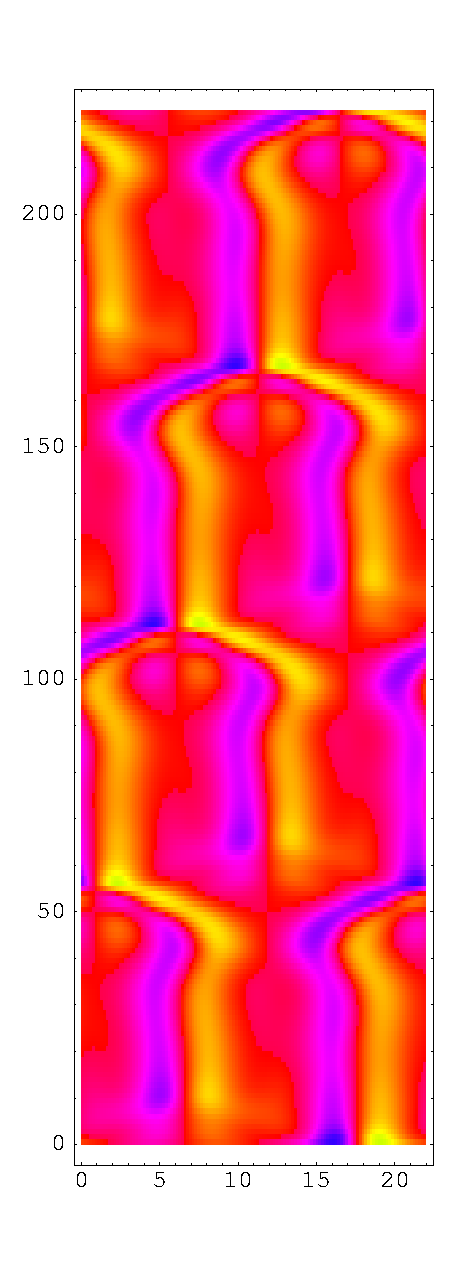
\includegraphics[width=2.5cm]{figs/rpo22-55-4-u.eps}
\hspace{0.1in}
\caption{
 The \rpo\ {\nameit}55 in $u(x,t)$ representation. 
        }
\label{f:rpo55u}
\end{figure}
%%%%%%%%%%%%%%%%%%%%%%%%%%%%%%%%%%%%%%%%%%%%%%%%%%%%%%%%%%%%%%%%%%


%%%%%%%%%%%%%%%%%%%%%%%%%%%%%%%%%%%%%%%%%%%%%%%%%%%%%%%%%%%%%%%%
\begin{figure}[t] %[h]
\centering
(a) 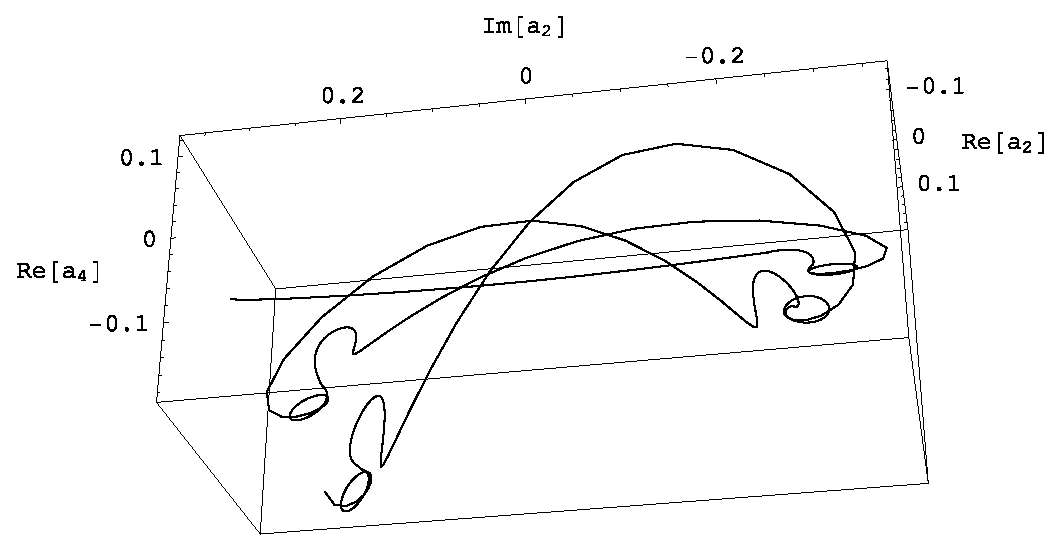
\includegraphics[width=8.0cm]{figs/rpo22-55-4-clean.eps}
% ./removecache.sh rpo22-55-4.eps
% abandoned rpoEq22-55-4.eps with mean velocity equilibrium embeded.
%
\hspace{0.1in}
(b) 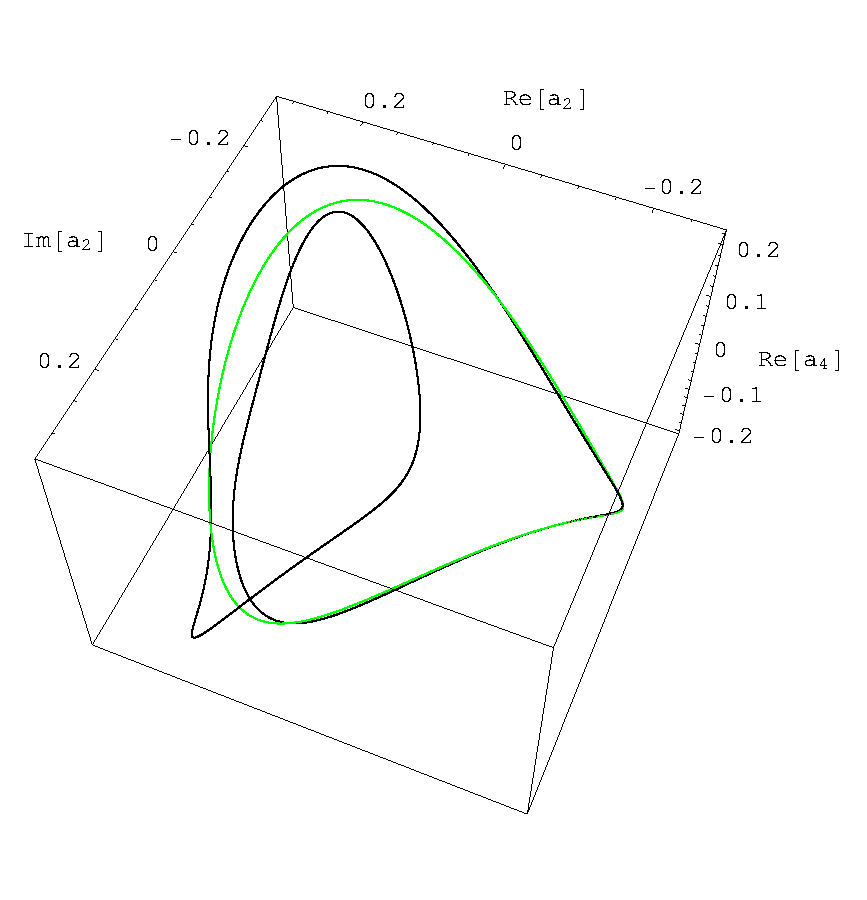
\includegraphics[width=6.0cm]{figs/rpoEq22-55-4-cm.eps}
\\
(c) [create rpoEq22-55-4-cm-?.eps]
\caption{
 The \rpo\ {\nameit}55 in: 
 (a) Phase space, traced for four periods $\period{p}$.
% Green curve belongs to \reffig{f:rpo55}(b) % rpo22-55-4-cm.eps
% rather than to  \reffig{f:rpo55}(a), % rpoEq22-55-4.eps?
 (b) mean velocity frame. 
        The continuos family of 
	equilibria A obtained by the action of $g$ is shown in green,
	the SA family shown in red. The \rpo\ {\nameit}55 stays close
	to either A or SA for close to 1/2 of equilibrum rotation
	period, then quickly jumps to the other equilibrium point.
 (c) mean velocity frame A, SA and {\nameit}55 projected on the 
	$[a_?,a_?]$ plane,
	with the $\sigma x = -x$ symmetry of \KSe\ explicit.
        }
\label{f:rpo55}
\end{figure}
%%%%%%%%%%%%%%%%%%%%%%%%%%%%%%%%%%%%%%%%%%%%%%%%%%%%%%%%%%%%%%%%%%


The two equilibria
capture qualitatively the mean velocity frame \rpo\ {\nameit}55 shape,
which follows the
equilibrium for most of the time, except for a quick swing where it
sidesteps by $d/4$, just as it does in \reffig{f:rpo55}. 

Please also plot it in plane, chose small Fourier coefficients
 which respect the $x \to -x$ symmetry of \KSe.
Then the symmetry of 2 mean velocity
equilibria and self-dual symmetry of \rpo\ {\nameit}55 will be explicit.

Eigenvalues of \rpo\ {\nameit}55 $g\jMps$: are
\\
$(-57.17,  1.00009, 1.00001, -0.500, -0.012, \cdots)$ .
%
%  Eigenvalues of the Jacobian without rotation
%  84.15, -33.86 + 28.94 i, c.c. , 0.48, 0.00019
% no good - missing marginal ones

There are two
marginal eigenvalues, one for time translation, one for
rotational invariance. 
The sign of $\ExpaEig_{1}=-57$ says this is a Moebius-kind orbit,
inverse hyperbolic.
Lyapunov $\Lyap=0.07$ says that this neighborhood is much less repelling than
the central equilibrium A, a better candidate for being embedded into the
ergodic attractor.

The \rpo\ initial condition is
so accurate the orbit in \reffig{f:rpo55}(b)
start visibly deviating after retracing the loop 6.5 times.
% the largest unstable multiplier is 
% $-57.17$ per period of the orbit - error would grow to $\approx 60^7
% = 2,800,000,000,000$.

For the \rpo s the accuracy of Jacobian depends
on the time step size, and long runs are needed to refine the results

For a numerical check of the \rpo\ stability eigenvalues,
used two inital
points along an unstable eigenvector $\jEigvec{1}$
at radial distance  $\approx 10^{-4}$ from the \eqv\ {\nameit}2,
and the initial inter-point separation $\Delta(0) \approx 10^{-5}$.
Integrated for time equal to the period $\period{p}=26.3556$ as calculated from
the \jacobianM\ and computed the leading Lyapunov exponent from the ratio of
final to initial distance 
$\Lyap= {1 \over \period{}}\ln( \Delta(\period{})/\Delta(0))$.
Get
$\Delta(\period{})/\Delta(0) =39.01$,
$\Lyap=0.13902$, in agreement with the \eqv\ {\nameit}2 
expanding eigenvalue $\Lyap=0.13904$
\[
\ExpaEig_{radial} =  e^{\Lyap \period{}} =38.99
\,.
\]

% Ruslan L Davidchack, 	10 Jul 2006 
The orbit RLD found has period 60 
rather than 55.  Because it comes so close to the steady states, 
this is probably a numerical precision error.
\\
plots:
  76 rpo60fm23.jpg	\\
 909 rpo60fm23.emf	\\
 180 rpos1.jpg	\\
1594 rpos1.emf	\\


% Ruslan L Davidchack, 	10 Jul 2006 
(the 55 rpo, or whichever seems easiest to explain)
$\period{} = 59.89$,

$(\ExpaEig_i e^{\pm i\theta_i})=
(
 -27.03397007874626,
   9.34426620337976,
   1.00000000001351,
   0.99999999999986,
   0.99995607257578,
   0.72779991655606,
  -0.05018967056231,
   0.00015065158255,
)$

Note the 3rd nearly marginal eigenvalue 0.999956. What near
invariance does it come from? 

Why are none of the eigenvalues complex?

period 77 rpo jumps between the two steady states.
\\
plots:	\\
  84 rpo77fm23.jpg	\\
1133 rpo77fm23.emf	\\
 176 rpos2.jpg	\\
1594 rpos2.emf	\\


        \Preliminary{
% Siminos thesis summary
% $Author$ $Date$

When statistical assumptions do not hold and coherent
structures are present in extended systems
such as fluid flows, flame fronts and field theories
a dynamical description of turbulent phenomena becomes
necessary.
% Recent experimental and theoretical advances\rf{science04}
% support a dynamical vision of turbulence:
% For any finite  spatial resolution, a turbulent flow follows approximately for a finite time
% a pattern belonging to a { finite alphabet} of admissible patterns.
% The long term dynamics is a {walk through the space of these unstable patterns}.
% When statistical assumptions\rf{frisch} break down and large
% scale coherent structures are present, a dynamical description
% as a walk through a space of unstable patterns becomes natural.
% The question is how to characterize and classify such patterns?
Here we follow the seminal Hopf paper\rf{hopf48}, and  visualize
turbulence not as  a sequence of spatial snapshots in turbulent evolution,
but as a trajectory in an  $\infty$-$d$ \statesp\ in which an
instant in turbulent evolution is a {unique} point. In the dynamical systems approach,
theory of turbulence for a given system, with given boundary conditions,
is given by (a) the geometry of the \statesp\ and (b) the associated measure,
\ie, the likelihood that asymptotic dynamics visits a given \statesp\ region.

In this thesis this vision is pursued in the context of \KS\
system, one of the simplest physically interesting spatially
extended nonlinear systems. Relaxing the restriction of
previous studies\rf{LanThesis,Christiansen97} to discrete
symmetry invariant subspace a new challenge confronts our
attempt to elucidate the \statesp\ geometry. Continuous
symmetry, in the form of a subgroup of \On{n} acting on
\statesp, endows \statesp\ with additional structure.
Symmetry dictates the bifurcation structure and the type of
observed solutions. At the same time the notion recurrence becomes
relative: Not only do we have to identify points along the
orbit of the nonlinear group of time evolution but also points
along the orbit of the linear symmetry group. The latter
identification, termed symmetry reduction, although
conceptually simple as the group action is linear, is hard to
implement in practice. The high dimensionality of \statesp\
that results from truncation of a PDE is one of the reasons.
The second reason is that, for most interesting group actions,
the process introduces singularities in the structure of the
reduced \statesp.

Here we propose a procedure to efficiently project dynamics of
solutions computed in the original space to a reduced \statesp.
This is done in conjunction with eliminating time-translational
invariance with suitably chosen Poincar\'e sections to avoid
singularities while setting the stage to compute return maps
that describe how unstable manifolds of solutions organize the
flow. Simplifying the visualization of high-dimensional flows,
this procedure yields new insight into which solutions of \KSe\
are key to describing the geometry of \statesp. In context of
low-dimensional, strongly-contracting flows the procedure leads
to one-dimensional return maps that encapsulate all the
information about the dynamics.

            } %end \Preliminary{
        \begin{acknowledgments}
% ackn.tex
% $Author$ $Date$

We thank Y.~Lan for determining
the $L=22$ \EQV{1}~\eqv.

        \end{acknowledgments}

        \Preliminary{
% siminos/atlas/flotsam.tex    master file: main.tex
% $Author$ $Date$

\section{Flotsam}
\label{s:flotsam}

\subsection{Pipe flows}
\label{s:review}
% former siminos/atlas/review.tex    master file: main.tex

As long as one is focusing on a single solution of \NSe, there are many
excellent, physically insightful $3D$ visualizations of the flow:
velocity fields on flow sections, isovorticity surfaces, videos of the
flow, and so on. But today we own dozens of exact \eqv\ and \reqv\
solutions for a given turbulent flow, and we are commencing an exploration of
states of turbulent fluids in terms of the unstable \po\ solutions whose
number, as a function of the increasing period, is growing exponentially.
How are we to visualize \emph{the totality} of these solutions in one go?

The answer was given by \cite{hopf48}, who envisioned the function space
of {\NS} velocity fields as an infinite-dimensional \statesp\ $\pS$ in
which each instantaneous state of $3D$ fluid velocity field $\vec{u}(\bx)$ is
represented as a unique point $\ssp$. In our particular application we
can represent $\ssp = (\vec{u}_{nkm})$ as a vector whose elements are the
primitive discretization variables \refeq{pipeDiscr}. The $3D$ velocity
field given by $\vec{u}_{knm}(\zeit)$, obtained from integration of the
\NSe\ in time, can hence be seen as trajectory $\ssp(\zeit)$ in
$\approx 100,000$ dimensional space spanned by the free variables of our
numerical discretization, with the \NS\ equations \refeq{NavStokesDev}
rewritten as
\beq
   \dot{\ssp} = \vel(\ssp) ,
   \qquad
   \ssp(\zeit) = \ssp(0)
            + \int_0^\zeit \! \mathrm{d}\zeit' \, \vel(\ssp(\zeit'))
\,,
\ee{symbolicNS}
where the current state of the fluid $ \ssp(\zeit)$ is the time-$\zeit$
forward map of the initial fluid state  $\ssp(0)$.

In order to quantify whether two fluid states are close to or far from
each other, one needs a notion of distance between two points in
\statesp, measured here as
\beq
  \Norm{\ssp-\ssp'}^2  = \braket{\ssp-\ssp'}{\ssp-\ssp'} =
\frac{1}{V}
\int_\bCell \! d \bx \;
(\vec{u}-\vec{u}') \cdot (\vec{u}-\vec{u}')
\,.
\ee{innerproduct}
There is no compelling reason to use this {`energy norm'}, other than
that velocity fields is what is given in a numerical computation. What
norm one actually uses depends very much on the application.
Visualizations of trajectory \refeq{symbolicNS} are of necessity
projections onto two or three dimensions.

Recently, \cite{GHCW07} have shown that the dynamics of different regions
of {\statesp}, considered as a high-dimensional vector space,
can be elucidated more profitably by a computationally
straight\-forward sets of \emph{physical} coordinates. One identifies
several prominent states of the flow $\vec{u}_A$, $\vec{u}_B$, $\dots$, such as
{\eqv} states and their linearized stability eigenvectors, states in whose neighborhoods the
turbulent flow spends most of the time, and from them constructs, by
Gram-Schmidt or (anti)-symmetrizations, an orthonormal basis set
$\{\be_1, \be_2, \cdots, \be_n\}$. The evolving fluid state $\bu(\zeit)$
is then projected onto this basis using the inner product
\refeq{innerproduct},
\beq
\ssp(\zeit) =(\ssp_1, \ssp_2, \cdots, \ssp_n, \cdots)(\zeit)
    \,,\qquad
\ssp_n(\zeit) = \braket{\vec{u}(\zeit)}{\be_n}
\,.
\ee{intrSspTraj}
Low-dimensional projections of the flow can be viewed in any of the $2D$ planes
$(\ssp_m, \ssp_n)$ or in $3D$ perspective views $(\ssp_{\ell},\ssp_m,
\ssp_n)$. An example is the \reffig{f:MeanVelocityFrame} projection on
the $3$\dmn\ frame $\{{\be}_1,{\be}_2,{\be}_3\}$ defined in \refeq{FrenetFrame1}.
It is worth emphasizing that the method affords low-dimensional {\em
visualization} without any low-dimensional {\em modeling} or dimension
reduction; the dynamics are computed with fully-resolved direct numerical
simulations.

Such visualizations are a prerequisite to uncovering the
interrelations between (the infinite number of) invariant solutions, and
constructing symbolic dynamics partitions of \statesp\ needed for a
systematic exploration of turbulent dynamics, the key challenge that we
address here for the case of turbulent pipe flows.


\subsection{Symmetries of pipe flow}
\label{s:SymmPipe}
% former siminos/atlas/symm.tex



Let $\LieEl(\phi,\shift)$ be the shift operator such that $\LieEl(\phi,0)$
denotes an azimuthal rotation by $\phi$ about the pipe axis,
and $\LieEl(0,\shift)$ denotes the stream-wise translation by
$\shift$; let $\sigma$ denote reflection about the $\theta=0$ azimuthal
angle:
\bea
\LieEl(\phi,\shift) \, [u,v,w,p](r,\theta,z)
        & = & [u,v,w,p](r,\theta-\phi,z-\shift)
			  \continue
\sigma \, [u,v,w,p](r,\theta,z) \;\; & = & [u,-v,w,p](r,-\theta,z)
\label{pipeSymms}
\eea
%
The \NSe\ for pipe flow are equivariant under these transformations. The
symmetry group of stream-wise periodic pipe flow is thus $\Group =
\On{2}_\theta \times \SOn{2}_z = \Dn{1} \ltimes \SOn{2}_{\theta} \times
\SOn{2}_z$, where $\Dn{1} = \{ e,\, \sigma \}$ denotes azimuthal
reflection, $\ltimes$ stands for a semi-direct product (in general,
reflections and rotations do not commute), and the subscripts $z,\theta$
indicate stream-wise translation and azimuthal rotation respectively.

In the literature
(see, \eg\ \cite{Recke2010}) such \SOn{2} is often referred to as the
circle group $S^1$, also denoted `one-torus' $T^1$.

\section{How to slice}
\label{s:algorithm}

\refFig{fig:sliceimage}, new proposal: take points on the good,
    blue \po, run each along the group orbit until $\sspRSing \in S$
    where it intersects the \sliceBord, see \refeq{sspRSing}, and thus plot
    the border of where the local slice ends, once on the left, and once
    on the right of the {\template}. Catch - I have not thought this
    through, not sure that the condition \refeq{sspRSing} can be
    satisfied on every group orbit...

\subsection{Rotation into the \slice}

As long as the norm is discretization independent, the \slice\ condition
\refeq{PCsectQ0} is independent of the numerical representation $\ssp$ of
the flow $\vec{u}$, be it finite difference, spectral, and so on. The
slice condition is solved for $\shift$ every few time steps using
Newton's method, where a good initial guess for $\shift(\zeit)$ is
obtained from the previous value and $\dot{\shift}(\zeit)$.

To avoid this, a global
atlas has to be pieced together from local \slice\ charts, fixed by
a well-chosen set of
\template s $\slicep{}^{(j)}$.
Shifts $\shift_j(\zeit)$ are tracked for each local \slice\ chart $\pS{}^{(j)}$,
such that the next $\shift_{j+1}(\zeit)$ is selected at intersection with
$\pS{}^{(j+1)}$
to minimise $\Norm{{\ssp}-{\ssp_i}}$.

%\APW{111104 The first sentence requires simplifying!}
As group orbits % of compact Lie groups
are smooth manifolds, have natural linear
representations (under linear action of a symmetry group, \statesp\
decomposes into a sum over irreducible subspaces), and have natural local
coordinate frames (the group tangent, curvature Frenet-Serret frames
\refeq{FrenetFrame}), good \slice s should be easier to construct than
the elusive ``good'' Poincar\'e sections of the time-evolution flows.
Indeed, as a generic \slice\ \refeq{PCsectQ0} is the set of all
group-orbit points closest to a given {\template}, it slices the group
orbits of \emph{all} full \statesp\ points\rf{FrCv11}. However, for a
nonlinear flow, there is no single \slice\ that really does the job: our
\slice\ is locally a hyperplane, expected to be a good description of
solutions similar to a given {\template} in some open neighborhood. The
variational distance condition \refeq{PCsectQ0} is only an extremum
condition, and as the group orbits of highly nonlinear states are highly
contorted (see \reffig{fig:2830GO6}\,(b)), they can have many
extrema, and multiple sections by a \slice\ hyperplane. For example, an
\rpo\  torus is always intersected by a \slice\ hyperplane in two or more
sections, see \reffig{fig:sliceimage}.
    \PC{\refFig{fig:sliceimage}, new proposal: take points on the good,
    blue \po, run each along the group orbit until $\sspRSing \in S$
    where it intersects the \sset, see \refeq{sspRSing}, and thus plot
    the border of where the local slice ends, once on the left, and once
    on the right of the {\template}. Catch - I have not thought this
    through, not sure that the condition \refeq{sspRSing} can be
    satisfied on every group orbit...
    }


\subsection{Dynamically important solutions and Newton's method}
\label{s:reqva}

The way in which the \mslices\ enables to find initial
guesses for $(\vec{u}(0),\period{},\shift)$, is the main differences
between this study and the previous ones.

Here we take as initial guesses samples of nearly recurrent velocity
fields generated by long-time simulations of turbulent dynamics
\rf{pchaot,CviGib10}. The intent is to find the {\em dynamically most
important} solutions, by sampling the turbulent flow's natural measure.
In practice, sufficiently good full \statesp\ initial guesses for
$(\vec{u}(0),\period{},\shift)$ would be almost impossible to find.
Checking correlations between $\vec{u}(\zeit)$ and
$\LieEl(0,\shift)\,\vec{u}(\zeit-\period{})$ for each $\period{}$, and
more problematically, for all possible shifts $(\phi,\shift)$, is an
unrealistic task. The \mslices, however, enables us determine close
recurrences  from the symmetry-reduced time series, and locates the
dynamically most important solutions, \ie, those trajectories that are
most likely to be observed in a long-time turbulent simulation. The \rpo
s are reduced to \po s, whose unstable manifolds are much easier to track
in the \reducedsp. The \rpo\ shift $\shift$ is given by the
reconstruction equation, \refeq{reconstrEq}, or, in practice, by phase
shift $\shift(\period{})-\shift(0)$ accumulated by the intermediate
Newton steps that keep the orbit within the slice.

Without symmetry reduction, the detection of the nearest recurrence of a
state near a previous state, earlier on the the same trajectory, would
require the calculating the minimum over all possible shifts. Within the
symmetry-\reducedsp\ the determination of recurrences is simple, as the
slices are constructed by requiring that the slice points are the minimum
distance points between the group orbits of the two states.

% append.tex
%
% Predrag               jun 20 2006
% $Author$ $Date$

\appendix

\PublicPrivate{%
        }{% switch to Private:

\section{\KSe\ according to Evangelos}
\label{ap:rpo}

The \KSe\ % (KSe)
reads:
 \beq
  u_t=(u^2)_x-u_{xx}- u_{xxxx} \, ,
  \label{eq:KS}
 \eeq

 We assume periodic boundary conditions on the $x\in [0,2\pi \tilde{L}]$
 interval:
 \beq
   u(x+2\pi\tilde{L},t)=u(x,t) \, ,
 \eeq
 which allows a Fourier series expansion:
 \beq
  u(x,t)=\sum_{k=-\infty}^{+\infty} a_k (t) e^{ i k x / \tilde{L}} \, .
  \label{eq:Fourier}
 \eeq
 Since $u(x,t)$ is real,
 \beq
  a_{k}=a^*_{-k} \, .
  \label{eq:a*}
 \eeq
 Substituting \refeq{eq:Fourier} into \refeq{eq:KS} we get:
 \beq
  \dot{a}_k=(k/\tildeL)^2\left(1-(1/\tildeL)^2 k^2\right)a_k
        + i (k/\tildeL)  \sum_{m=-\infty}^{+\infty}a_m a_{k-m} \, .
  \label{eq:Fcoef}
 \eeq

 From \refeq{eq:Fcoef} we notice that $\dot{a}_0=0$ and thus $a_0$ is an integral
 of the equations or, from \refeq{eq:Fourier}, the average of the solution $\int dx u(x,t)$
 is a constant. Due to galilean invariance we may set $a_0=0$ without loss of generality
 and we only have to compute $a_k$'s with $k\geq 1$. % Explain this in detail somewhere.

 Truncating the infinite tower of equations by setting $a_k=0$ for $k>d$, using the identity $a_{-k}=a^*_k$ and splitting the
 resulting equations into real and imaginary part by setting $a_k=b_k+i c_k$, we have

 \bea
  \dot{b}_k & = & \left(\frac{k}{\tildeL}\right)^2\left(1- \left(k/\tildeL\right)^2 \right)b_k  \continue
    & & - \frac{k}{\tildeL} \left(\sum_{m=1}^{k-1}c_m b_{k-m}+\sum_{m=k+1}^{N}c_m b_{m-k}
                    -\sum_{m=1}^{N-k}c_m b_{k+m} \right)  \continue
    & & - \frac{k}{\tildeL} \left(\sum_{m=1}^{k-1}b_m c_{k-m}-\sum_{m=k+1}^{N}b_m c_{m-k}
                    +\sum_{m=1}^{N-k}b_m c_{k+m} \right)
  \label{eq:tmp:b-Trunc}
 \eea
 \bea
   \dot{c}_k & = & \left(\frac{k}{\tildeL}\right)^2\left(1- \left(k/\tildeL\right)^2 \right)c_k  \continue
    & & - \frac{k}{\tildeL}\left( \sum_{m=1}^{k-1}c_m c_{k-m}-\sum_{m=k+1}^{N}c_m c_{m-k}
                    -\sum_{m=1}^{N-k}c_m c_{k+m} \right)    \continue
    & & + \frac{k}{\tildeL} \left(\sum_{m=1}^{k-1}b_m b_{k-m}+\sum_{m=k+1}^{N}b_m b_{m-k}
                    +\sum_{m=1}^{N-k}b_m b_{k+m} \right)
   \label{eq:tmp:c-Trunc}
 \eea
 where now only terms $c_{k},b_{k}$ with $0<k<d$ appear. Observe
 \beq
    \sum_{m=1}^{N-k}c_m b_{k+m} = \sum_{m=k+1}^{N}b_m c_{m-k}\,,
 \eeq
 \etc and thus \refeq{eq:tmp:b-Trunc} and \refeq{eq:tmp:c-Trunc} simplify to
  \bea
  \dot{b}_k & = & \left(\frac{k}{\tildeL}\right)^2\left(1- \left(k/\tildeL\right)^2 \right)b_k  \continue
    & & - \frac{k}{\tildeL} \left(\sum_{m=1}^{k-1}c_m b_{k-m}-2\sum_{m=1}^{N-k}c_m b_{k+m} \right)  \continue
    & & - \frac{k}{\tildeL} \left(\sum_{m=1}^{k-1}b_m c_{k-m}+2\sum_{m=1}^{N-k}b_m c_{k+m} \right)
  \label{eq:b-Trunc}
 \eea
 \bea
   \dot{c}_k & = & \left(\frac{k}{\tildeL}\right)^2\left(1- \left(k/\tildeL\right)^2 \right)c_k  \continue
    & & - \frac{k}{\tildeL}\left( \sum_{m=1}^{k-1}c_m c_{k-m}-2\sum_{m=1}^{N-k}c_m c_{k+m} \right)  \continue
    & &  +\frac{k}{\tildeL}\left( \sum_{m=1}^{k-1}b_m b_{k-m}+2\sum_{m=1}^{N-k}b_m b_{k+m} \right)\,.
   \label{eq:c-Trunc}
 \eea

 We begin by calculating the matrix of variations $A_{ij} \equiv \frac{\partial v_i(x)}{\partial x_j}$ for the antisymmetric
 subspace for which $b_k=0, c_{-k}=-c_{k}$ and thus
 \beq
       \dot{c}_k =  \left(\frac{k}{\tildeL}\right)^2\left(1- \left(k/\tildeL\right)^2 \right)c_k
            - \frac{k}{\tildeL}\left( \sum_{m=1}^{k-1}c_m c_{k-m}
                            -2\sum_{m=1}^{N-k}c_m c_{k+m} \right)   \,.
 \eeq

 Then
 \bea
    \frac{\partial \dot{c}_k}{\partial c_{j}}  =
        \left(\frac{k}{\tildeL}\right)^2\left(1- \left(k/\tildeL\right)^2 \right) \delta_{kj}
            - \frac{k}{\tildeL}\frac{\partial}{\partial c_j}\left( \sum_{m=1}^{k-1}c_m c_{k-m}-2\sum_{m=1}^{N-k}c_m c_{k+m} \right) \,.
 \eea
 Concider the second term:
 \bea
    - \frac{k}{\tildeL}\frac{\partial}{\partial c_j}\left( \sum_{m=1}^{k-1}c_m c_{k-m}-2\sum_{m=1}^{N-k}c_m c_{k+m} \right) & = &
        - \frac{k}{\tildeL} \sum_{m=1}^{k-1} \left(\delta_{m,j} c_{k-m}+c_m \delta_{k-m,j} \right) \continue
                        & & + 2 \frac{k}{\tildeL}\sum_{m=1}^{N-k} \left(\delta_{m,j} c_{k+m}+c_m \delta_{k+m,j}\right)
 \eea
 We need to consider two cases separately:
 \begin{itemize}
    \item $k\leq j$
        \bea
             -\frac{k}{\tildeL}\frac{\partial}{\partial c_j}\left( \sum_{m=1}^{k-1}c_m c_{k-m}-2\sum_{m=1}^{N-k}c_m c_{k+m} \right) & = &
                    -\frac{k}{\tildeL}( 0+0 ) + 2\frac{k}{\tildeL} (c_{k+j} + c_{j-k}) \continue
                & = &   2 \frac{k}{\tildeL} (c_{k+j}-c_{k-j})
        \eea
    \item $k > j$
        \bea
             -\frac{k}{\tildeL}\frac{\partial}{\partial c_j}\left( \sum_{m=1}^{k-1}c_m c_{k-m}-2\sum_{m=1}^{N-k}c_m c_{k+m} \right) & = &
                    -\frac{k}{\tildeL}(c_{k-j} + c_{k-j} ) + 2\frac{k}{\tildeL} (c_{k+j}  + 0 ) \continue
                & = &  2 \frac{k}{\tildeL} (c_{k+j}-c_{k-j})
        \eea
 \end{itemize}
 and thus
 \beq
    \frac{\partial \dot{c}_k}{\partial c_{j}} =  \left(\frac{k}{\tildeL}\right)^2\left(1- \left(k/\tildeL\right)^2 \right)\delta_{kj} + 2 \frac{k}{\tildeL} (c_{k+j}-c_{k-j})
 \eeq

 For the case of the full space we need to consider the four matrices $\frac{\partial \dot{b}_k}{\partial b_j},\frac{\partial \dot{b}_k}{\partial c_j},\frac{\partial \dot{c}_k}{\partial b_j},\frac{\partial \dot{c}_k}{\partial c_j}$. Following the above procedure
 \beq
    \frac{\partial \dot{c}_k}{\partial b_{j}} =  2 \frac{k}{\tildeL} ( b_{k+j}+b_{k-j} )\,,
 \eeq
 \beq
    \frac{\partial \dot{b}_k}{\partial b_{j}} =  \left(\frac{k}{\tildeL}\right)^2\left(1- \left(k/\tildeL\right)^2 \right)\delta_{kj} - 2 \frac{k}{\tildeL} (c_{k+j} + c_{k-j}) \,,
 \eeq
 \beq
    \frac{\partial \dot{b}_k}{\partial c_{j}} = 2 \frac{k}{\tildeL} (b_{k+j}-b_{k-j}) \,.
 \eeq


\section{\KS\ according to Ruslan}
The \KSe\ has a slightly different form:
\begin{equation}
  u_t=-{\textstyle\frac{1}{2}}(u^2)_x-u_{xx}- u_{xxxx} \, ,
\end{equation}
which can be reduced to Eq.~(\ref{eq:KS}) by the transformation $u
\rightarrow -2u$.

The \KSe\ in terms of Fourier modes:
\begin{equation}
  \hat{u}_k \equiv {\cal F}[u]_k = \frac{1}{L}\int_0^L u(x,t) e^{-ikx/\tilde{L}}dx\,,
  \qquad u(x,t) \equiv {\cal F}^{-1}[\hat{u}] = \sum_{k\in{\mathbb Z}} \hat{u}_k e^{ikx/\tilde{L}}
\end{equation}
 is given by
\begin{equation}
  \dot{\hat{u}}_k =[(k/\tildeL)^2-(k/\tildeL)^4]\hat{u}_k -
  \frac{ik}{2\tilde{L}}{\cal F}[({\cal F}^{-1}[\hat{u}])^2]_k\,.
\end{equation}
Since $u$ is real, the Fourier modes are related by $\hat{u}_{-k} =
\hat{u}^\ast_k$.

The above system is truncated as follows: The Fourier transform
${\cal F}$ is replaced by its discrete equivalent
\begin{equation}
  a_k \equiv {\cal F}_N[u]_k = \sum_{n = 0}^{N-1} u(x_n)
  e^{-ikx_n/\tilde{L}}\,,\qquad u(x_n) \equiv {\cal F}_N^{-1}[a]_n
  = \frac{1}{N}\sum_{k = 0}^{N-1} a_k e^{ikx_n/\tilde{L}}\,,
\end{equation}
where $x_n = 2\pi\tilde{L}n/N$ and $a_{N-k} = a^\ast_k$.  Since $a_0
= 0$ due to galilean invariance and setting $a_{N/2} = 0$ (assuming
$N$ is even), the number of independent variables in the truncated
system is $N-2$.  The truncated system looks as follows:
\begin{equation}
  \dot{a}_k =[(k/\tildeL)^2-(k/\tildeL)^4]a_k -
  \frac{ik}{2\tilde{L}}{\cal F}_N[({\cal F}_N^{-1}[a])^2]_k\,.
\end{equation}
with $k = 1,\ldots,N/2-1$, although in the Fourier transform we need
to use $a_k$ over the full range of $k$ values from 0 to $N-1$.

The discrete Fourier transform ${\cal F}_N$ can be computed by FFT.
In Fortran and C, the routine {\tt REALFT} from Numerical Recipes
can be used.  In Matlab, it is more convenient to use complex
variables for $a_k$.  Note that Matlab function {\tt fft} is, in
fact, the inverse Fourier Transform.

To derive the equation for the matrix of variations, I use the fact
that ${\cal F}_N$ is a linear operator.  Since we need to
differentiate separately with respect to the real and imaginary
components of $a_k$, I use the notation $a_k = b_{2k-1} + ib_{2k}$.
\begin{equation}
  \frac{\partial \dot{a}_k}{\partial b_j} =
  [(k/\tildeL)^2-(k/\tildeL)^4]\delta_{kj} -
  \frac{ik}{\tilde{L}}{\cal F}_N[{\cal F}_N^{-1}[a]\cdot{\cal
  F}_N^{-1}[\delta_{kj}]]\,,\quad j = 1,\ldots,N-2
\end{equation}
where the dot indicates componentwise product, and the inverse
Fourier transform is applied separately to each column of
$\delta_{kj}$. Here, $\delta_{kj}$ is not a standard Kronecker
delta, but a complex valued $N\times N-2$ matrix:
\begin{equation}
  \delta_{kj} = \left(
  \begin{array}{ccccc}
  0 &  0 & 0 &  0 &\cdots\\
  1 &  i & 0 &  0 &\cdots\\
  0 &  0 & 1 &  i &\cdots\\
\multicolumn{5}{c}\dotfill \\
  0 &  0 & 0 &  0 &\cdots\\
\multicolumn{5}{c}\dotfill \\
  0 &  0 & 1 & -i &\cdots\\
  1 & -i & 0 &  0 &\cdots\\
  \end{array}  \right),
\end{equation}
with index $k$ running from 0 to $N-1$.  I admit, the notations are
a bit stretched here, but I find them convenient when coding this
equation using FFT.

\section{Tales from the Literature}

\subsection{\KSe\ according to Kuramoto and Sivashinsky}

The original form in which \KSe was derived (in $1-D$) was (up to scaling factors):
\beq
	y_t=-y_{xxxx}-y_{xx}-\frac{1}{2}y_x^2\,,
	\label{eq:KSeOR}
\eeq
with periodic boundary conditions in the $(0,L)$ interval. The equation we are using
differs in the nonlinear term:
\beq 
	u_t=-u_{xxxx}-u_{xx}-uu_x\,.
	\label{eq:KSeAP}
\eeq
It can be obtained from \refeq{eq:KSeOR} by setting $u=y_x$. The two equations are used interchangeably
and referred to as \KSe. The authors of \refref{TsveTri89} state that the solutions of the two equations
differ considerably despite the simple way they are related. 

\subsection{\KSe according to Greene and Kim}

Greene and Kim \refref{ksgreene88} use the following form of \KSe:
\beq
	y_t=-4y_{xxxx}-\alpha\left(y_{xx}+\frac{1}{2}y_x^2-\frac{1}{4\pi}\int_0^{2\pi}y_x^2\ dx\right)\,,
	\label{eq:KSeGreeneKim}
\eeq
where $\alpha$ the bifurcation parameter and periodic boundary conditions are assumed in the $(0,2\pi)$
interval. To see its relation to our form of the equation, first take the derivative of \refeq{eq:KSeGreeneKim}
with respect to $x$ and then make the substitution $y_x=u$ to obtain
\beq
	u_t=-4u_{xxxx}-\alpha\left(u_{xx}+uu_x\right)\,.
\eeq
Rescale according to
\beq
	\tilde{x}=\frac{\alpha^{1/2}}{2} x
	\label{eq:GKxScale}
\eeq
\beq
	\tilde{t}=\frac{\alpha^2}{4} t
\eeq
\beq
	\tilde{u}=\frac{2}{a^{1/2}} u
\eeq
to obtain \refeq{eq:KSeAP}. From \refeq{eq:GKxScale} we see that our control parameter $\tilde{L}=L/2\pi$ is connected
to $\alpha$ through $\frac{\alpha^{1/2}}{2}$. Thus our system size $L=22.0$ corresponds to $\alpha=49.0395$.

%%%%%%%%%%%%%%%%%%%%%%%%%%%%%%%%%%%%%%%%%%%%%%%%%%%%%%%%%%%%%%%%
\begin{figure}[t]
	% \vspace*{-5pt}
\centering
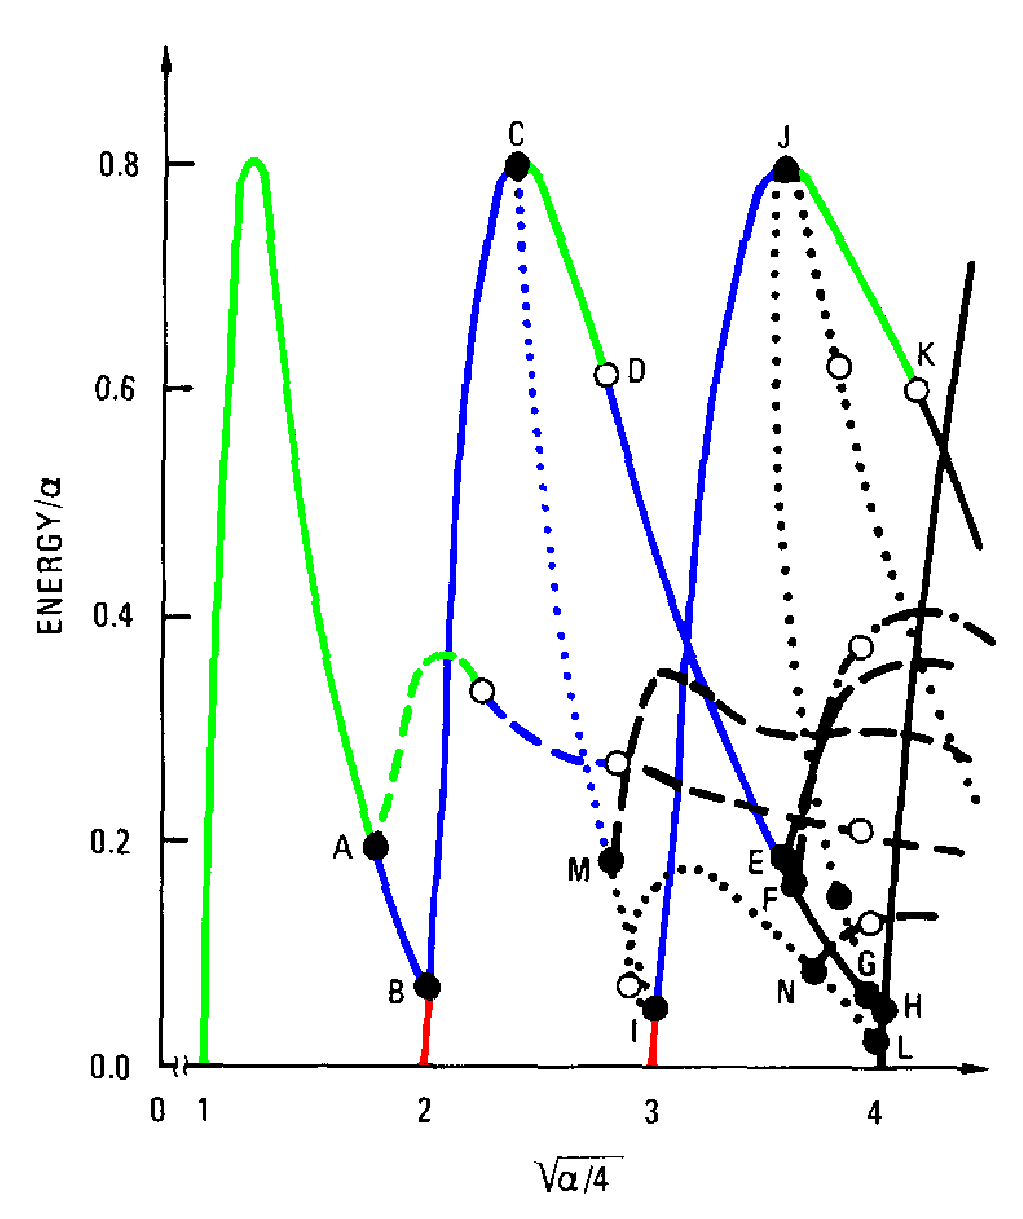
\includegraphics[width=0.5\textwidth]{figs/GreeneKimBifColor.eps}
	% \vspace*{-5pt}
\caption{
	{\small
The energy of steady states as a function of the bifurcation
parameter a. The solid curves are N-cell solutions,
dotted curves are for GLMRT, the dash-dotted curve is for the
giant states, and dashed curves are for the propagating solutions.
Open circles are for Hopf bifurcation. From \refref{ksgreene88}. Here
we've color-coded the branches to reflect the number of unstable
eigenvalues (or complex pairs). Red: 2 unstable eigenvalues, Blue: 1
unstable eigenvalue, Green: stable. Regions that could not be
resolved with the help of \refref{ksgreene88} or are of no interest
to our present purposes have been left black.
        } %end \small
        }
\label{fig:GreeneKim}
	% \vspace*{-5pt}
\end{figure}
%%%%%%%%%%%%%%%%%%%%%%%%%%%%%%%%%%%%%%%%%%%%%%%%%%%%%%%%%%%%%%%%%%

Greene and Kim systematically study the steady states of \KSe\ and their bifurcations, extending the work of
previous authors, \refrefs{Mks86,laquey74}. We review their bifurcation diagram, \reffig{fig:GreeneKim}, up to
the system size that we use. They define the energy as
\beq
	E=\frac{1}{2\pi}\int_0^{2\pi}y_x^2\, dx\,.
\eeq
Since $u=y_x$ we have from \refeq{eq:stdks} that $c\sim E$. 

For small $\alpha$ the only equilibrium state of the system is the trivial state, $y(x,t)=0$, which is
stable for $\tilde{L}=(a/4)^{1/2}<1$. At $\tilde{L}=N$, with $N$ integer, the $N$'th harmonic becomes unstable and
the trivial state bifurcates to the so called $N$-cell states. These states contain only the multiples of the $N$'th
harmonic, i.e. only the components $a_N,a_{2N},...$ in our notation. 
Moreover, the $N$-cell states are found to be symmetric (in our case, since $u=y_x$ they will be
antisymmetric). In general Greene and Kim show that symmetric solutions are not traveling. 
At point $A$ in \reffig{fig:GreeneKim} the $1$-cell state loses stability and bifurcates to a stable, 
asymetric traveling wave solution, which later on becomes unstable through a Hopf bifurcation. 

At $\tilde{L}=(a/4)^{1/2}=2$ the system has become large enough that a $2$-cell steady state appears. At point $B$
in \reffig{fig:GreeneKim} the $1$-cell branch merges to the $2$-cell branch. In general each $N$-cell branch merges to the corresponding $2N$-cell branch.

At point $C$ in \reffig{fig:GreeneKim} the $2$-cell state bifurcates to a type of equilibrium solution
found by La Quey, Mahajan, Rutherford and Tang, \refref{laquey74} and generalized by Greene and Kim who refer to them as GLMRT equilibria. GLMRT solutions are symmetric (u(x) is antisymmetric) and can be roughly described as long-wave distorted $N$-cell states.

The last type of solution identified in \refref{ksgreene88} appears at point $F$ in \reffig{fig:GreeneKim} and is termed
giant state. because its amplitude grows as the system size increases.

According to the bifurcation diagram \reffig{fig:GreeneKim}, at the point that corresponds to our system size $\tilde{L}=\frac{\alpha^{1/2}}{2}=3.501$ the steady states we should expect are the $2$- and $3$-cell states ($\EQV{2}$ and $\EQV{3}$ respectivelly), the GLMRT state that bifurcates from a $3$-cell state at point $I$ ($\EQV{1}$) and the traveling waves that belong to the branches starting at points $A$ ($\REQV{\pm}{1}$) and $M$ (not identified yet).
 
        }% end \PublicPrivate

            } %end \Preliminary{

\PC{PC.bib is temporary, eventually incorporate into ../bibtex/siminos.bib}
\bibliography{../bibtex/siminos,PC}

\end{document}
